%!TEX root = ../thesis.tex
%*******************************************************************************
%*********************************** Fourth Chapter *****************************
%*******************************************************************************
%*******************************************************************************
\chapter{Kernel-based central tendency estimation}
%*******************************************************************************
\hfill
\localtableofcontents
\newpage

%\section{Kernel discrepancy}
%\section{Quantization with kernel herding \elias{SIAM UQ talk 2022, RENEW cpaper 2022}}
%\section{Bayesian quadrature \elias{otkerneldesign package}}
%\section{Numerical experiments \elias{ctbenchmark package}}
%\section{Application to wind turbine mean fatigue estimation \contrib{DCE paper}}

%============================================================%
\section{Introduction}
%============================================================%
As a sustainable and renewable energy source, offshore wind turbines (OWT) are likely to take a growing share of the global electric mix. 
However, to be more cost-effective, wind farm projects tend to move further from the coast, exploiting stronger and more regular wind resources. 
Going further offshore, wind turbines are subject to more severe and uncertain environmental conditions (i.e., wind and waves). 
In such conditions, their structural integrity should be certified. To do so, numerical simulation and probabilistic tools have to be used. 
In fact, according to \cite{graf_2016}, for new environmental conditions or new turbine models, international standards such as \cite{iec_2019} from the International Electrotechnical Commission and \cite{dnv_loads_2016} from Det Norske Veritas recommend performing over 200,000 simulations distributed over a grid. 
Numerical simulations are computed by a costly hydro-servo-aero-elastic wind turbine model, making the design process time-consuming. 
In the following, the simulated output cyclic loads studied are aggregated over the simulation period to assess the mechanical fatigue damage at hot spots of the structure. 
To compute the risks associated with wind turbines throughout their lifespan, one can follow the steps of the universal framework for the treatment of uncertainties \citep{rocquigny_2008} presented in \fig{fig:UQ}. 
After defining the problem (Step A), one can quantify the uncertainties related to site-specific environmental conditions denoted by the random variable $\bX$ (Step B). 
Then, one can propagate them through an OWT simulation model $g(\cdot)$ (Step C), and estimate a relevant quantity of interest $\psi(Y) = \psi(g(\bX))$ (e.g., mean, quantile, failure probability). 
A proper estimation of the quantity relies on a good uncertainty model and an efficient sampling method to estimate the quantity of interest.

\begin{figure}[!h]
    \centering
    %\begin{figure}[h]
%    \centering
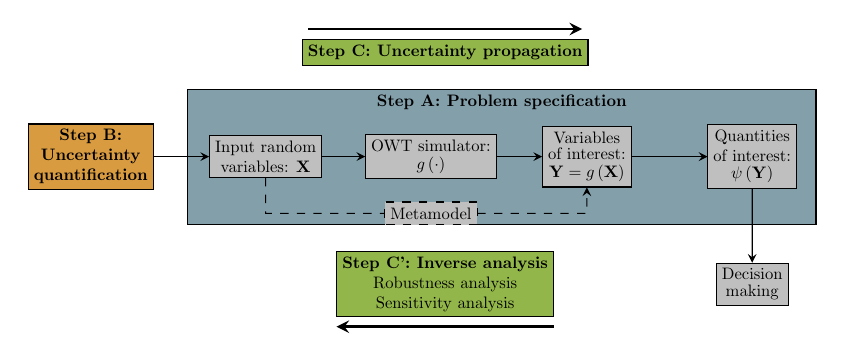
\begin{tikzpicture}[scale=0.6, every node/.style={transform shape}]
    \node[rectangle,draw,fill=YellowOrange!70!gray] (a) at (-9,0) {\shortstack{\textbf{Step B:} \\ \textbf{Uncertainty} \\ \textbf{quantification}}};
\node[rectangle,draw,fill=YellowGreen!70!gray] (f) at (-1.5,2.2) {
\textbf{Step C: Uncertainty propagation}};
\node[rectangle,draw,fill=YellowGreen!70!gray] (g) at (-1.5,-2.7) {\shortstack{
\textbf{Step C': Inverse analysis} \\ Robustness analysis \\ Sensitivity analysis}};
\node[rectangle,draw,minimum width=13.3cm,fill=SkyBlue!40!gray] (h) at (-0.3,0) {\shortstack{\textbf{Step A: Problem specification} \\ \phantom{a} \\ \phantom{a} \\ \phantom{a} \\ \phantom{a} \\ \phantom{a} \\ \phantom{a} \\ \phantom{a} \\ \phantom{a} \\ \phantom{a} }};
\node[rectangle,draw,fill=lightgray] (b) at (-5.3,0) {\shortstack{
Input random \\ variables: $\mathbf{X}$}};
\node[rectangle,draw,fill=lightgray] (c) at (-1.8,0) {\shortstack{
OWT simulator: \\$g\left(\cdot\right)$}};
\node[rectangle,draw,fill=lightgray] (d) at (1.5,0) {\shortstack{
Variables \\ of interest: \\ $\mathbf{Y}=g\left(\mathbf{X}\right)$}};
\node[rectangle,draw,fill=lightgray] (e) at (5,0) {\shortstack{
Quantities \\ of interest: \\ $\psi \left(\mathbf{Y}\right)$}};
\node[rectangle,draw,fill=lightgray, dashed] (i) at (-1.8,-1.2) {Metamodel};
\node[rectangle,draw,fill=lightgray] (j) at (5,-2.7) {\shortstack{Decision \\ making}};
\draw[-stealth, black, line width=1pt] (-4.4,2.7) -- (1.4,2.7);
\draw[-stealth, black, line width=1pt] (0.8,-3.6) -- (-3.8,-3.6);
\draw[-stealth, black] (a) -- (b);
\draw[-stealth, black] (b) -- (c);
\draw[-stealth, black] (c) -- (d);
\draw[-stealth, black] (d) -- (e);
\draw[-stealth, black, dashed] (b) -- (-5.3,-1.2) -- (i) -- (1.5,-1.2) -- (d);
 \draw[-stealth, black] (e) -- (j);

\end{tikzpicture}
%    \caption{General uncertainty quantification and propagation framework}
%    \label{Fig:UQ}
%\end{figure}
    \caption{General uncertainty quantification and propagation framework (adapted from \cite{ajenjo_2023})}
    \label{fig:UQ}
\end{figure}

The uncertainties related to the OWT environment follow a joint distribution with a complex dependence structure. 
This challenging distribution has been fitted with different parametric approaches in the literature (step B in \fig{fig:UQ}), mainly using conditional distributions \citep{vanem_fekhari_2023}, but also vine copulas \citep{li_zhan_2020}. 
When one has access to data, another way is to directly use the data as empirical representation of input uncertainties. 

These uncertainties have then been propagated to fatigue damage (the output), making it random, and to the associated quantities of interest (step C in \fig{fig:UQ}). 
When uncertainty propagation aims at central tendency studies, the methods employed are split into two groups. 
Methods of the first group rely on numerical integration by Monte Carlo sampling \citep{graf_2016}, quasi-Monte Carlo sampling \citep{muller_cheng_2018}, or deterministic quadrature rules \citep{bos_2020}. 
All these methods estimate the quantity directly on the numerical simulator's outputs. 
Methods of the second group use metamodels (or surrogate models) to emulate the costly numerical model by a statistical model such as polynomial chaos expansion \citep{dimitrov_kelly_2018, murcia_dimitrov_2018}, Gaussian processes \citep{huchet_2019,slot_sorensen_2020,wilkie_galasso_2021}, or artificial neural networks \citep{aoues_2023}. 

When uncertainty propagation aims at studying the tail of the output distribution (e.g., reliability analysis), one can estimate a quantile or a failure probability. 
Failure probabilities were studied, in static reliability analysis \citep{zwick_muskulus_2015,slot_sorensen_2020,wilkie_galasso_2021} or time-dependent reliability analysis \citep{abdallah_lataniotis_2017,lataniotis_2019}. 
To get a better understanding of the OWT numerical models behavior, authors have used sensitivity analysis methods \citep{daveiga_iooss_2021}, which determine the most influential inputs on the damage (step C' in \fig{fig:UQ}). 
Among others, one can cite the application of Spearman's rank correlation coefficients and Morris method's by \cite{verlade_kramhoft_2019,petrovska_2022}, the direct calculation of Sobol' indices after fitting a polynomial chaos model by \cite{murcia_dimitrov_2018} and the use of Kullback-Leibler divergence by \cite{teixeira_oconnor_2017}. 
Each of those methods brings something different to the analysis.

This paper will focus on central tendency estimation (i.e., $\psi(\bX) = \E(\bX)$) by: (1) direct sampling on the numerical model, (2) sampling on a static regression model, or (3) sampling on an active regression model (i.e., observations of the numerical model are progressively added to enhance a goal-oriented metamodel). 
In the specific context of wind turbines, this paper explores how to study the central tendency study of the fatigue damage output, by carrying out the uncertainty propagation of a complex input joint distribution through a costly wind turbine simulator. 
This work proposes a new approach for given data, fast, and fully-distributable uncertainty propagation for OWT models. 
Overall, this paper reviews the methods of Bayesian quadrature and presents its application on the industrial wind turbines case.
%Considering that this simulator is often deployed on a high-performance computing facility, this 
%\elias{What is the paper's goal? How to realize the central tendency study of the output fatigue damage, by carrying out the uncertainty propagation of a complex input distribution through costly wind turbine simulation model.}
In this paper, Section 2 will detail the industrial use-case related to a wind farm operating in Teesside, UK. 
Then, Section 3 will introduce different methods for central tendency estimation. 
Section 4 will analyze the results of numerical experiments on analytical and industrial cases. 
Then, the last section will present discussions and conclusions.

%============================================================%
\section{Treatment of uncertainties on the Teesside wind farm}\label{sec1}
%Teesside offshore wind farm use-case
%From environmental uncertainties to wind turbine fatigue assessment
%============================================================%

An OWT is a complex system interacting with its environment. 
To simulate the response of this system against a set of environmental solicitations, multi-physics numerical models are developed. 
In our case, it is a chain of three numerical codes executed sequentially. 
As illustrated in \fig{fig:bloc_diagram}, a simulation over a time period is the sequence of (1) turbulent wind speed field generation, (2) wind turbine simulation (computing various outputs including mechanical stress), and (3) post-processing to assess the fatigue damage of the structure.
\begin{figure}[!h]
\begin{center}
    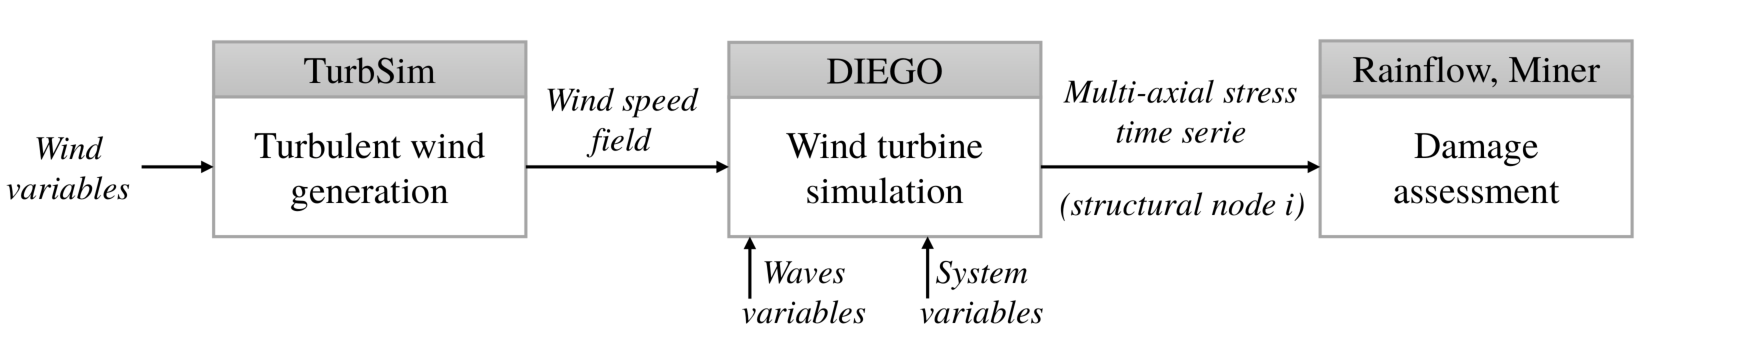
\includegraphics[width=0.8\linewidth]{part2/figures/DCE/simulator_blocs.pdf}    
\end{center}
\caption{Diagram of the chained OWT simulation model}
\label{fig:bloc_diagram}
\end{figure}

\begin{table*}[h]
    \centering
    \caption{Teesside Offshore Wind turbine datasheet}
    \begin{tabular}{ll}
     \hline
     \multicolumn{2}{l}{Siemens SWT-2.3–93} \\ \hline
        Rated power & 2.3 MW\\
        Rotor diameter & 93 m\\
        Hub height & 83 m\\
        Cut-in, cut-out wind speed & 4 m/s, 25 m/s\\\hline
    \end{tabular}
    \label{tab:owt_datasheet}
\end{table*}


%------------------------------------------------------------%
\subsection{Numerical simulation model}
%------------------------------------------------------------%
This section describes more precisely the modeling hypotheses considered in this case. 
Starting from the turbulent wind field simulator TurbSim (developed by \cite{turbsim_2009} from the National Renewable Energy Laboratory, USA) that uses a Kaimal spectrum \citep{kaimal_1972}. 
To extrapolate the wind speed vertically, the shear is modeled by a power law. 
Since the wind field generation shows inherent stochasticity, each 10-minute long simulation is repeated with different pseudo-random seeds and the average damage over these repetitions is studied. 
This question was widely studied by some authors, (e.g., \cite{slot_sorensen_2020}), who concluded that the six repetitions recommended by the \cite{iec_2019} are insufficient to properly average this stochasticity. 
In the following, the simulations are repeated eleven times (allowing direct access to the median value). 
This number of repetitions was chosen as a compromise between the general number of simulations and the storage capacity of the generated simulations.

DIEGO (for ``Dynamique Intégrée des Éoliennes et Génératrices Offshore\footnote{In english, ``Integrated Dynamics of Wind Turbines and Offshore Generators''.}'') is a code developed by EDF R\&D \citep{kim_natarajan_2022} to simulate the aero-hydro-servo-elastic behavior of OWTs. 
It takes the turbulent wind speed field generated by TurbSim as input and computes the dynamical behavior of the system (including the multiaxial mechanical stress at different nodes of the structure). 
For our application, the control system is modeled by the open-source DTU controller \citep{dtu_controler_2013}, and no misalignment between the wind and the OWT is assumed. 
As for the waves, they are modeled in DIEGO using a JONSWAP spectrum (named after the 1975 Joint North Sea Wave Project). 
Our study uses a DIEGO model of a Siemens SWT 2.3MW bottom-fixed turbine on a monopile foundation (see the datasheet in Table \ref{tab:owt_datasheet}), currently operating in Teesside, UK (see the wind farm layout and wind turbine diagram in \fig{fig:teesside_layout}). 
Although wind farms are subject to the wake effect, affecting the behavior and performance of some turbines in the farm, this phenomenon is not considered in the following. 
To avoid numerical perturbations and reach the stability of the dynamical system, our simulation period is extended to 1000 seconds and the first 400 seconds are cropped in the post-processing step. 
This chained OWT numerical simulation model has been deployed on an EDF R\&D HPC facility to benefit from parallel computing speed up (a single simulation on one CPU takes around 20 minutes).

\begin{figure}[!h]
\begin{center}
    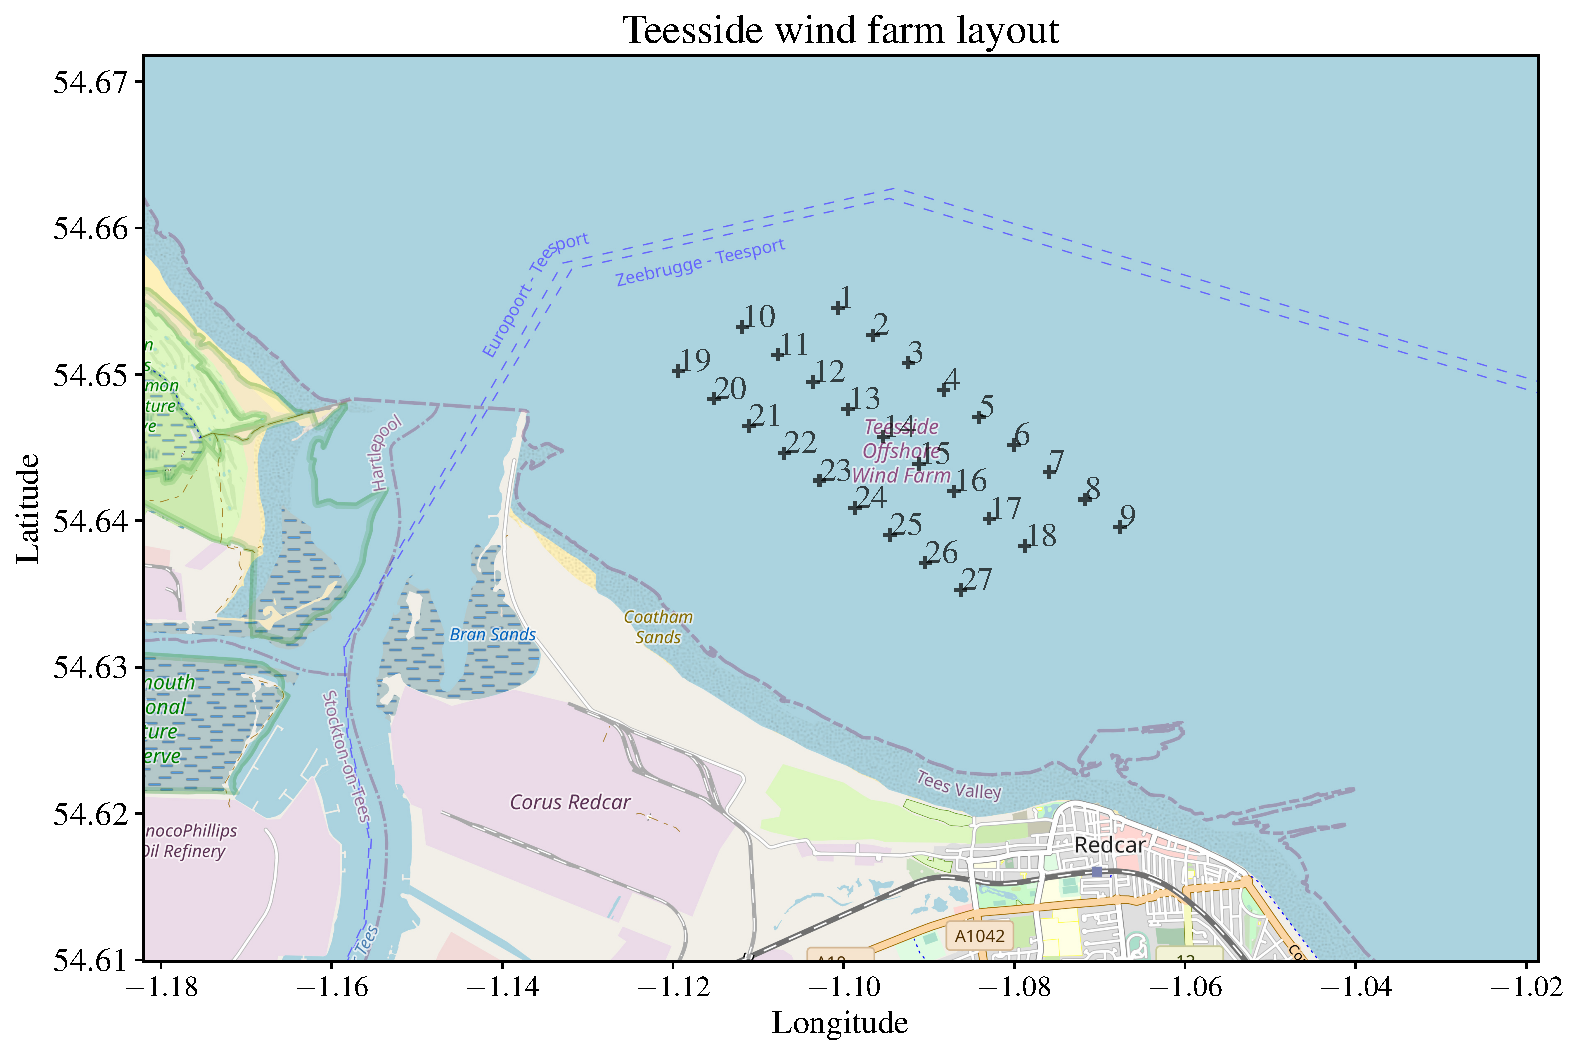
\includegraphics[width=0.6\linewidth]{part2/figures/DCE/teesside/map_teesside_layout.pdf}
    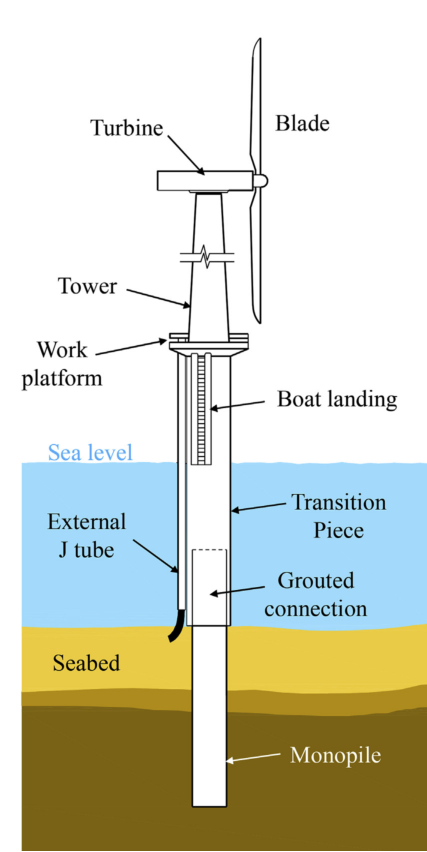
\includegraphics[width=0.25\linewidth]{part2/figures/DCE/teesside/owt_diagram.pdf}
\end{center}
\caption{Teesside wind farm layout (left). Monopile OWT diagram \citep{Chen_2018_owt_diagram} (right)\label{fig:teesside_layout}}
\end{figure}

%------------------------------------------------------------%
\subsection{Measured environmental data}
%------------------------------------------------------------%
During the lifespan of a wind farm project, environmental data is collected at different phases. 
In order to decide on the construction of a wind farm, meteorological masts and wave buoys are usually installed on a potential site for a few years. 
After its construction, each wind turbine is equipped with monitoring instruments (e.g., cup anemometers). 
In total, five years of wind data have been collected on the turbines which are not affected by the wake on this site. 
Their acquisition system (usually called SCADA, for ``Supervisory Control And Data Acquisition'') have a sampling period of ten minutes. 
The wave data arise from a buoy placed in the middle of the farm. This data describes the physical features listed in Table \ref{tab:envi_variables}.

The farm of Teesside is located close to the coast, making the environmental conditions very different depending on the direction (see the wind farm layout in \fig{fig:teesside_layout}). 
Since measures are also subject to uncertainties, a few checks were realized to ensure that the data were physically consistent. 
The truncation bounds defined in Table \ref{tab:envi_variables} were applied since this study is not interested in extreme values but in central tendency estimation (i.e., mean behavior). 
In addition, a simple trigonometric transform is applied to each directional feature to take into account their cyclic structure. 
Finally, the remaining features are rescaled (i.e., using a min-max normalization). 
The matrix plot of the transformed data in \fig{fig:envi_pairplot} is an innovative plot named \emph{copulogram}. 
A copulogram is an innovative plot as it decomposes the data between the effects of the marginals and those of the dependence between features. 
To do so, it represents the marginals with univariate kernel density estimation plots (diagonal), and the dependence structure with scatter plots in the ranked space (upper triangle). 
On the bottom triangle the scatter plots are set in the physical space, gathering the effects of the marginals and the dependencies. 
Since the dependence structure is theoretically modeled by an underlying copula, this plot is called \emph{copulogram}, generalizing the well-known ``correlogram'' to nonlinear dependencies. 
It gives a synthetic and empirical decomposition of the dataset.

On \fig{fig:envi_pairplot}, a large sample $\iS$ (with a size $N=10^4$) is randomly drawn from the entire Teesside data (with size $N_{\mathrm{Teesside}} = 2\times 10^5$), and plotted in grey. 
In the same figure, the orange matrix plot is a subsample of the sample $\iS$, selected by kernel herding, a method that will be presented in Section 3. 
Visually, this orange subsample seems to match the original sample both in terms of marginal distributions and dependence structure. 
In the following study, the large samples $\iS$ will be considered as an empirical representation of the multivariate environmental distribution $\bX \in \iD_{\bX} \subset \R^p$, of density $f_{\bX}$, and called \textit{candidate set}. 
Contrarily to parametric approaches which can be used to describe the joint environmental uncertainty, this method intends to directly subsample from this large and representative dataset. 
This technique samples a joint distribution without modeling it. Indeed, a proper parametric model fit would be challenging for complex dependence structures such as the one plotted on \fig{fig:envi_pairplot}. 
\cite{li_zhan_2020} built a parametric model of a similar multivariate distribution using vine copulas. 
Alternatively, a nonparametric approach coupling empirical Bernstein copula fitting with kernel density estimation of the marginals is introduced in Section \ref{sec:ebc}.

\begin{table*}[h] \caption{Description of the environmental data.}
\begin{center}
%\tabletext{
\begin{tabular*}{\textwidth}{@{\extracolsep\fill}llll@{}}\hline
Variable & Notation & Unit & Description\\
\hline
Mean wind speed & $U$ & $\mathrm{m.s^{-1}}$ & 10-min. average horizontal wind speed\\
Wind turbulence & $\sigma_U $ & $\mathrm{m.s^{-1}}$ & 10-min. wind speed standard deviation\\
Wind direction & $\theta_{wind} $ & deg. &  10-min. average wind direction\\
Significant wave height & $H_s $ & m & Significant wave height\\
Peak wave period & $T_p $  & $\mathrm{s}$ & Peak 1-hour spectral wave period \\
Wave direction & $\theta_{wave} $ & deg. &  10-min. average wave direction\\
\hline
\end{tabular*}
\label{tab:envi_variables}
%}
\end{center}
\end{table*}

\begin{figure}[!h]
\begin{center}
    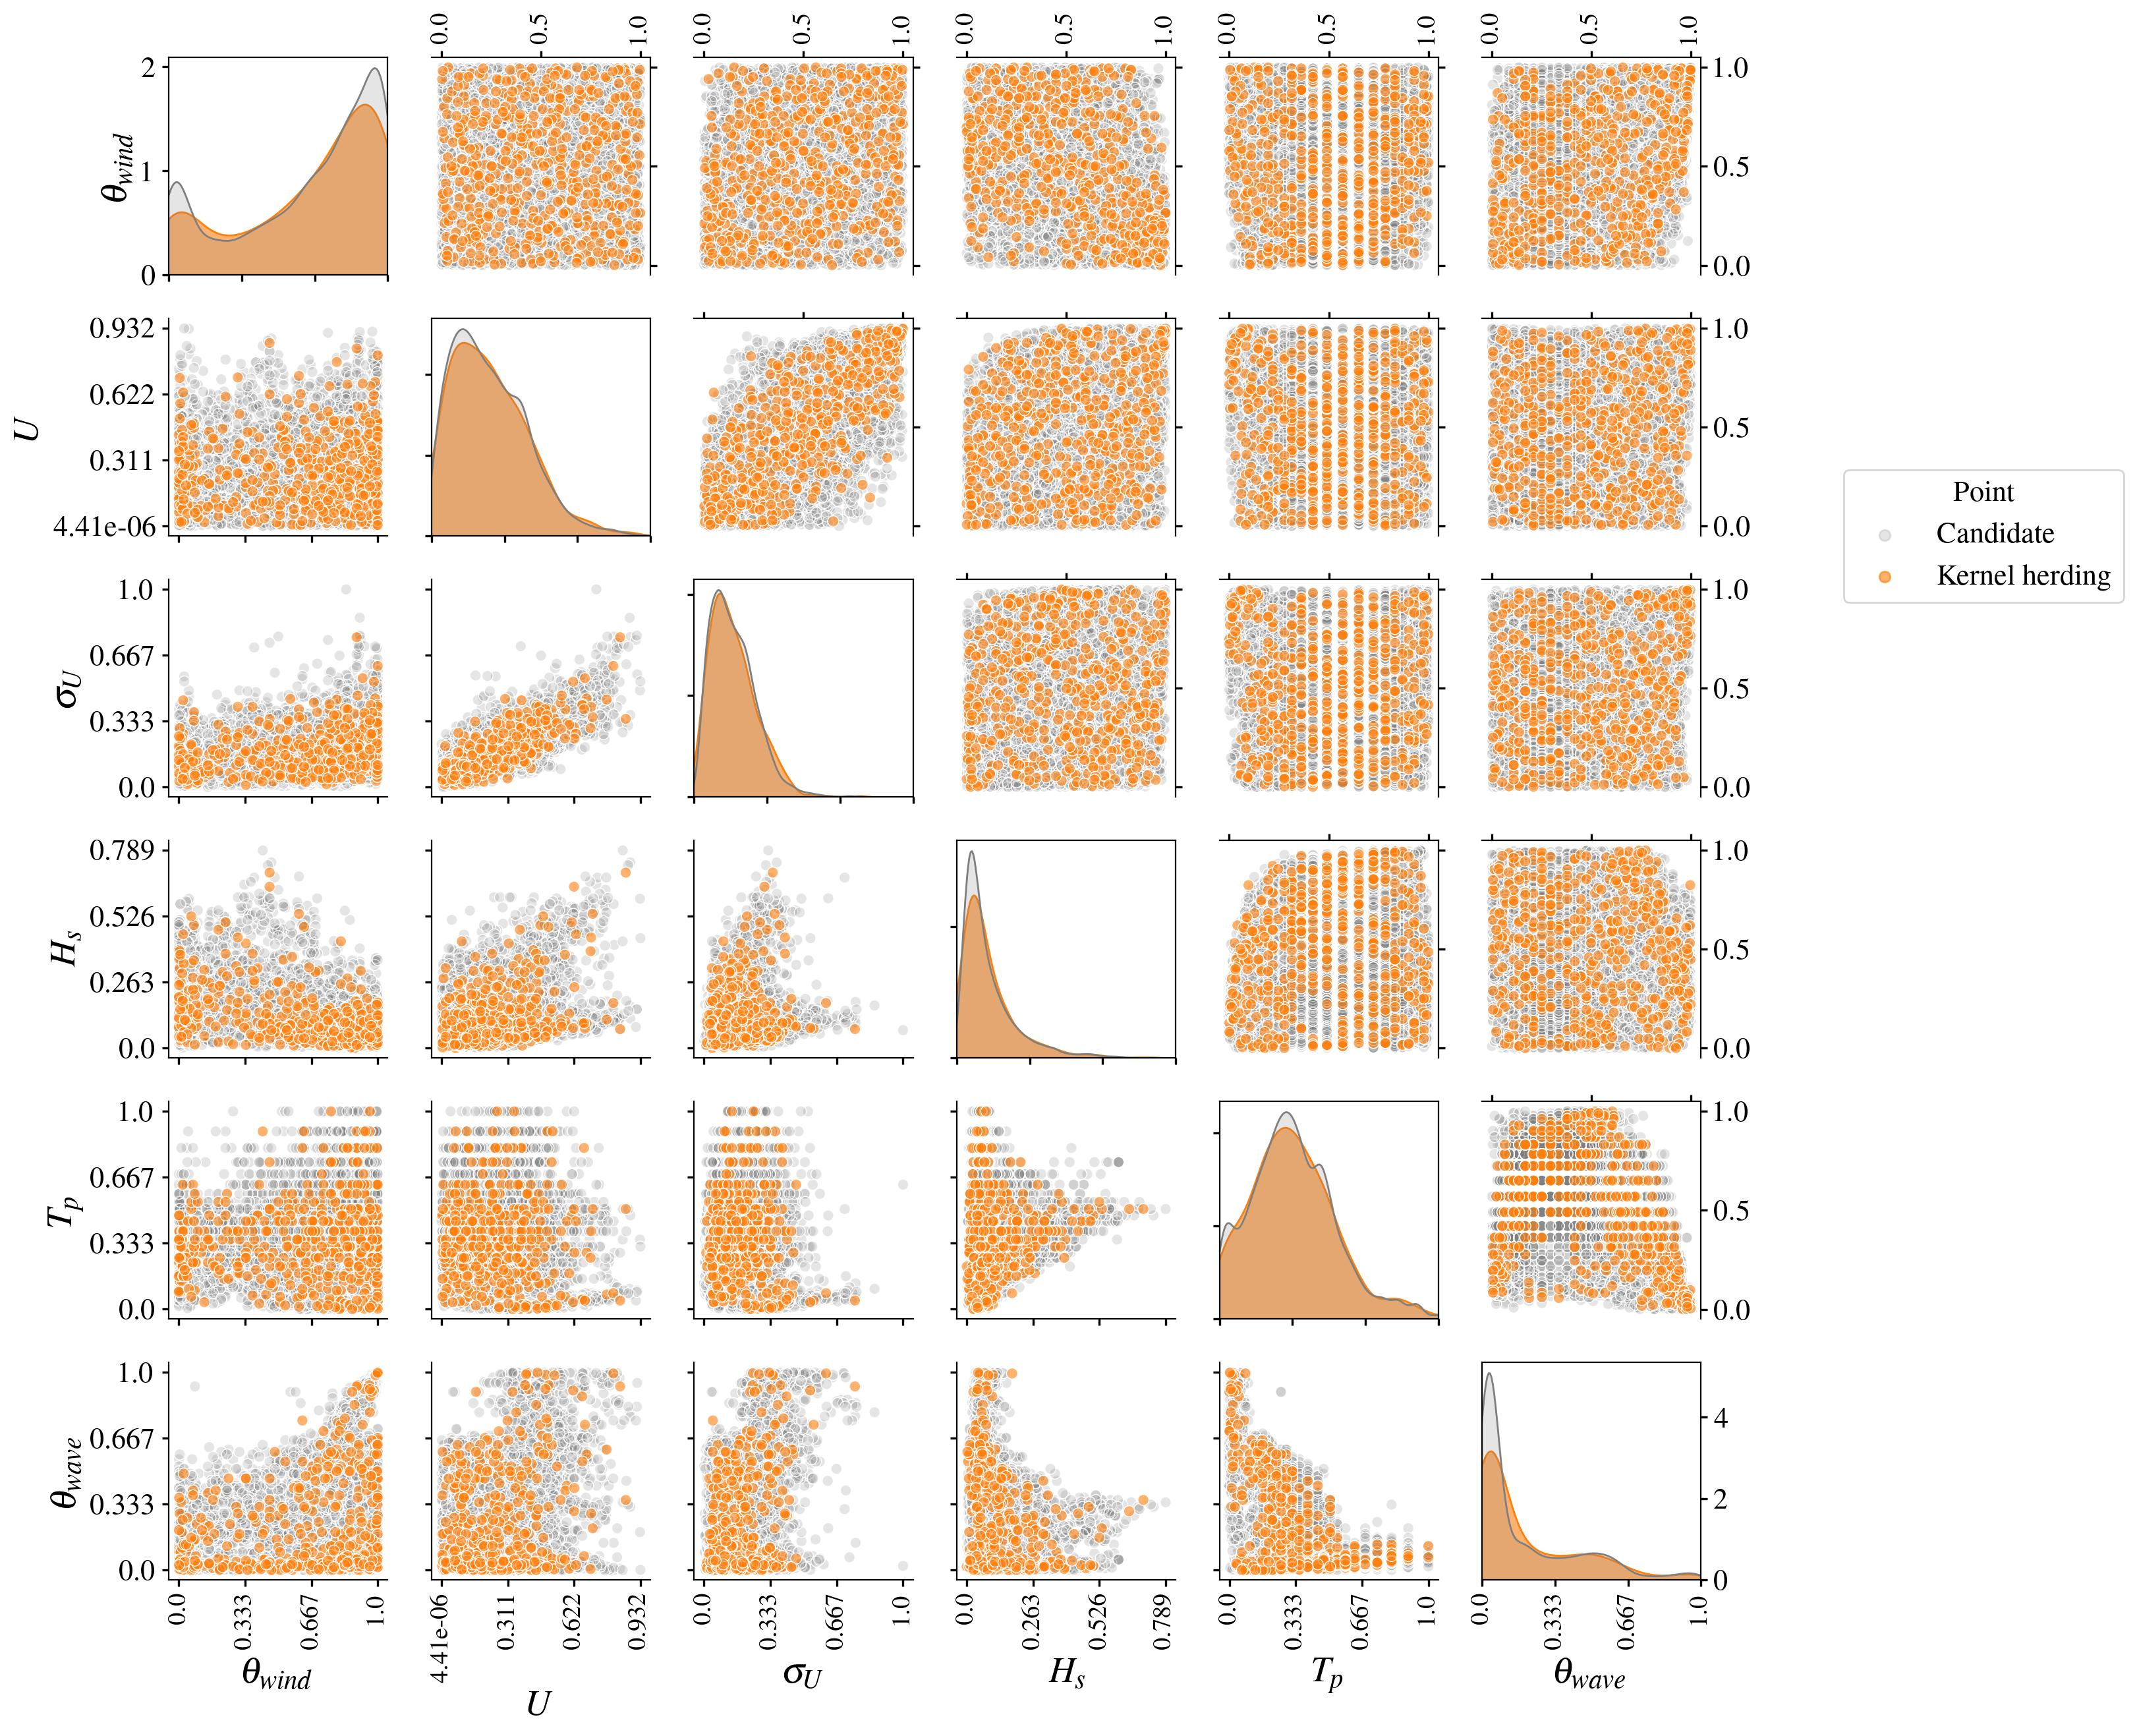
\includegraphics[width=\linewidth]{part2/figures/DCE/teesside/pairplot_kh.jpg}    
\end{center}
\caption{Copulogram of the Teesside measured data ($N=10^4$ in grey), kernel herding subsample ($n=500$ in orange). 
Marginals are represented by univariate kernel density estimation plots (diagonal), the dependence structure with scatter plots in the ranked space (upper triangle). 
Scatter plots on the bottom triangle are set in the physical space\label{fig:envi_pairplot}}
\end{figure}

%------------------------------------------------------------%
\subsection{Non parametric fit with empirical Bernstein copula}\label{sec:ebc}
%------------------------------------------------------------%
The  Sklar theorem \citep{joe_1997} states that the multivariate distribution of any random vector $\mathbf{X} \in \R^p$ can be broken down into two objects:
\begin{enumerate}
    \item A set of univariate marginal distributions to describe the behavior of the individual variables;
    \item A function describing the dependence structure between all variables, called a copula.
\end{enumerate}
This theorem states that considering a random vector $\mathbf{X} \in \R^p$, with its distribution $F$ and its marginals $\{F_i\}_{i=1}^p$, there exists a copula $C: [0, 1]^p \rightarrow [0, 1]$, such that:
\begin{equation}
    F(x_1, \dots, x_p) = C\left(F_1(x_1), \dots, F_p(x_p)\right). 
\end{equation}

It allows us to divide the problem of fitting a joint distribution into two independent problems: fitting the marginals and fitting the copula. 
Additionally, when the joint distribution is continuous, this copula is unique. 
Copulas are continuous and bounded functions defined on a compact set (the unit hypercube). 
Bernstein polynomials allow to uniformly approximate as closely as desired any continuous and real-valued function defined on a compact set (Weierstrass approximation theorem). 
Therefore, they are good candidates to approximate unknown copulas. 
This concept was introduced as \textit{empirical Bernstein copula} (EBC) by \cite{sancetta_satchell_2004} for applications in economics and risk management. 
Later on, \cite{segers_2017} offered further asymptotic studies. Formally, the multivariate Bernstein polynomial for a function $C: [0, 1]^p \rightarrow \R$ on a grid over the unit hypercube $G:=\left\{\frac{0}{h_1}, \dots, \frac{h_1}{h_1}\right\} \times \dots \times \left\{\frac{0}{h_p}, \dots, \frac{h_p}{h_p}\right\}, \mathbf{h} = (h_1, \dots, h_p) \in \N^p$, is written as follows: 

\begin{equation}
    B_{\mathbf{h}}(C)(\bu) := \sum_{t_1=0}^{h_1} \dots \sum_{t_p=0}^{h_p} C\left(\frac{t_1}{h_1}, \dots, \frac{t_p}{h_p}\right) \prod_{j=1}^p P_{h_j, t_j}(u_j),\label{eq:ebc_chap4}
\end{equation}
with $\bu = (u_1, \dots, u_p) \in [0, 1]^p$, and the Bernstein polynomial $P_{h, t}(u):= \frac{t!}{h!(t-h)!}u^h(1-u)^{t-h}$. When $C$ is a copula, then $B_{\bm}(C)$ is called ``Bernstein copula''. 
Therefore, the empirical Bernstein copula is an application of the Bernstein polynomial in \eq{eq:ebc_chap4} to the so-called ``empirical copula''. 
In practice, considering a sample $\bX_n = \left\{\bx^{(1)}, \dots, \bx^{(n)}\right\} \in \R^{np}$ and the associated ranked sample $\bR_n = \left\{\br^{(1)}, \dots, \br^{(n)}\right\}$, the corresponding empirical copula is written: 

\begin{equation}
    C_n(\bu) := \frac1n \sum_{i=0}^{n} \prod_{j=1}^{p} \1 \left\{ \frac{r_j^{(i)}}{n} \leq u_j \right\}, \bu = (u_1, \dots, u_p) \in [0, 1]^p.
\end{equation}

Provided a large enough learning set $\bX_n$, the EBC combined with kernel density estimation for the marginals fit well the environmental joint distribution related to the dataset in \fig{fig:envi_pairplot}. 
Moreover, the densities of the EBC are available in an explicit form, making Monte Carlo or quasi-Monte Carlo generation easy. 
For a thorough presentation of this method and theoretical results regarding the EBC tuning, see the manuscript of \cite{lasserre_2022}. 
Further discussions and numerical experiments on the estimation of nonparametric copula models are presented in \cite{nagler_2017}. 


%%%%%%%%%%%%%%%%%%%%%%%%%%
%\textcolor{red}{
%for $\mathbf{u}\in[0,1]^d$, where $r_j^i=\lceil binNumber U_j^i \rceil$, $binNumber - r_j^i + 1$, $(\mathbf{U}_i)_{i=1,\dots,N}$ is the empirical copula sample associated to sample and $I_{a,b}(x)$ is the value of the regularized incomplete beta function of parameters $a$ and $b$ at $x$. This construction leads to an actual copula if and only if $N$ is a multiple of $binNumber$. If it is not the case, the last points of the sample are dropped in order to fulfill this condition.
%Where N is The number of cells into which each dimension of the unit cube $[0, 1]^d$ is divided to cluster the empirical copula sample.}
%%%%%%%%%%%%%%%%%%%%%%%%%
%% Note and implementation
%For a thorough presentation of this method, see the manuscript of \cite{lasserre_2022}. %Moreover, the EBC was implemented in OpenTURNS, a Python package for the treatment of uncertainties \cite{baudin_2016}.
%% Section goal
%This section introduces a non-parametric alternative method to fit multivariate distributions: the empirical Bernstein copula. This tool was first introduced by \cite{sancetta_satchell_2004}, mostly for applications in economics and risk management. This section will illustrate the use of EBC on the previously introduced environmental data set. The aim is twofold, first to explore how well this tool can fit such data, second to examine how sensitive this method is to the data (especially regarding extreme behavior). 
%
%Finally, the empirical Bernstein copula offers a lot of advantages to fit a complex multivariate distribution. Using a non-parametric method is at the same time straightforward and practical. This empirical copula directly fits the dimension of the input data set, while parametric copulas are mostly bivariate. On the downside, EBC is subject to the curse of dimensionality, however, it scales better than other non-parametric methods, such as kernel density estimation (whose performance significantly deteriorates with the input dimension). Applied to this data set, the empirical Bernstein copula is efficient and offers a lot of flexibility.

%------------------------------------------------------------%
\subsection{Fatigue assessment}
%------------------------------------------------------------%
As described in \fig{fig:bloc_diagram}, a typical DIEGO simulation returns a 10-minute multiaxial stress time series at each node $i \in \N$ of the 1D meshed structure. 
Since fatigue laws are established for uniaxial stresses, the first step is to compute one equivalent Von Mises stress time series at each structural node.

However, the foundation and the tower of an OWT are a succession of tubes with various sections connected by bolted or welded joints. 
Our work studies the welded joints at the mudline level, identified as a critical area for the structure. 
To compute fatigue in this joint, the external circle of the welding ring is discretized for a few azimuth angles $\theta \in \R_+$ (see the red points in the monopile cross-section on the right in \fig{fig:wind_wave_roses}). 
The equivalent Von Mises stress time series is then reported on the external welding ring for an azimuth $\theta$. 
According to \cite{li_zhan_2020} and our own experience, the most critical azimuth angles are roughly aligned with the main wind and wave directions (whose distributions are illustrated in \fig{fig:wind_wave_roses}). 
According to these illustrations, the wind and wave conditions have a very dominant orientation, which is explained by the closeness of the wind farm to the shore. 
Then, it is assumed that azimuth angles in these directions will be more solicited, leading to higher fatigue damage. 
To assess fatigue damage, rainflow counting \citep{dowling_1972} first identifies the stress cycles and their respective amplitudes (using the implementation of the ASTM E1049-85 rainflow cycle counting algorithm from the Python package \texttt{rainflow}\footnote{\url{https://github.com/iamlikeme/rainflow}}). 
For each identified stress cycle of amplitude $s$, the so-called ``Stress vs. Number of cycles'' curve (also called the ``W\"ohler curve'') allows one to estimate the number $N_{\mathrm{c}}$ of similar stress cycles necessary to reach fatigue ruin:
\begin{equation}
    N_{\mathrm{c}} := W(s) = a s^{-m}, \, a\in\R, \, m\in\R.
    \label{eq:wohler}
\end{equation}

Finally, a usual approach to compute the damage is to consider the fatigue contribution of each stress cycle identified using Miner's rule. 
Damage occurring during a 10-minute operating time is simulated and then scaled up to the OWT lifetime. 
More details regarding damage assessment are available in Appendix \ref{apx:fatigue}. 
For a realization of environmental conditions $\bx \in \iD_{\bX}$, at a structural node $i$, an azimuth angle $\theta$; $k$ stress cycles of respective amplitude $\{s_{i, \theta}^{(j)}(\bx)\}_{j=1}^k$ are identified. 
Then, Miner's rule \citep{fatemi_1998} defines the damage function $g_{i, \theta}(\bx): \iD_{\bX} \rightarrow \R_+$ by:
\begin{equation}
    g_{i, \theta}(\bx) = \sum_{j=1}^{k} \frac{1}{N_{\mathrm{c}}^{(j)}} = \sum_{j=1}^{k} \frac{1}{W\left(s_{i, \theta}^{(j)}(\bx)\right)}.
    \label{miner1}
\end{equation}

As defined by the DNV standards for OWT fatigue design \citep{dnv_fatigue_2016}, the quantity of interest in the present paper is the ``mean global damage'' $d_{i, \theta}$, computed at the node $i$, for an azimuth angle $\theta$:
\begin{equation}
    d_{i, \theta} = \E[g_{i, \theta}(\bX)] = \int_{\iD_\bX} g_{i, \theta}(\bx) f_{\bX}(\bx)\, \d \bx \,.
    \label{eq:mean_integral}
\end{equation}

To get a preview of the distribution of this output random variable $g_{i, \theta}(\bX)$, a histogram of a large Monte Carlo simulation ($N_{\mathrm{ref}}=2000$) is represented in \fig{fig:histo_mc} (with a log scale). 
The log-damage presents a little asymmetry,so it is unlikely to be normally distributed.
%\begin{equation}
%    ln(Y_{i, \theta}) \sim \iN(\mu, \sigma) \Leftrightarrow
%    Y_{i, \theta} \sim \mathcal{LN}(\mu, \sigma); \qquad
%    \E[Y_{i, \theta}] = \exp\left(\mu + \frac{\sigma^2}{2}\right)
%\end{equation}

\begin{figure}[!h]
\begin{center}
    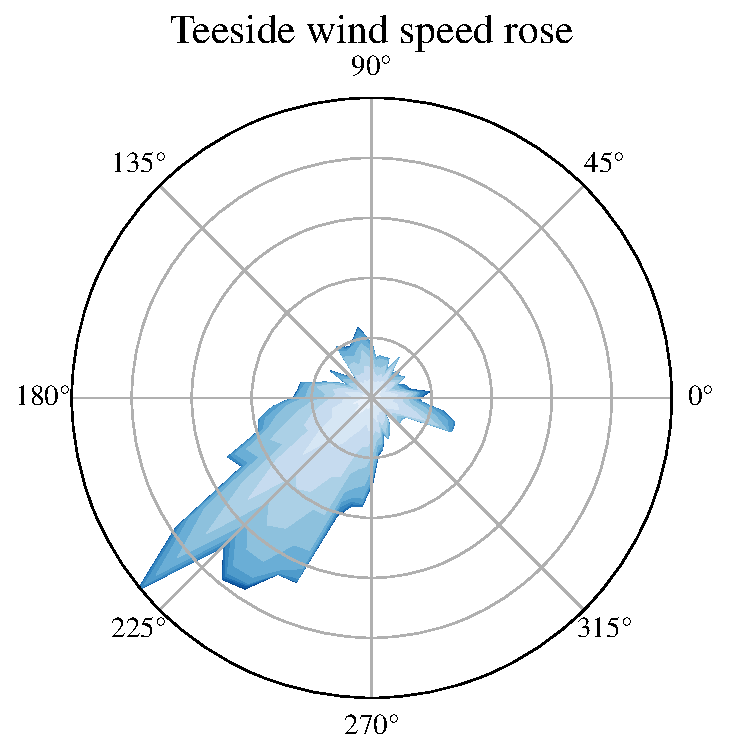
\includegraphics[width=0.3\textwidth]{part2/figures/DCE/teesside/teeside_wind_rose.pdf} \quad
    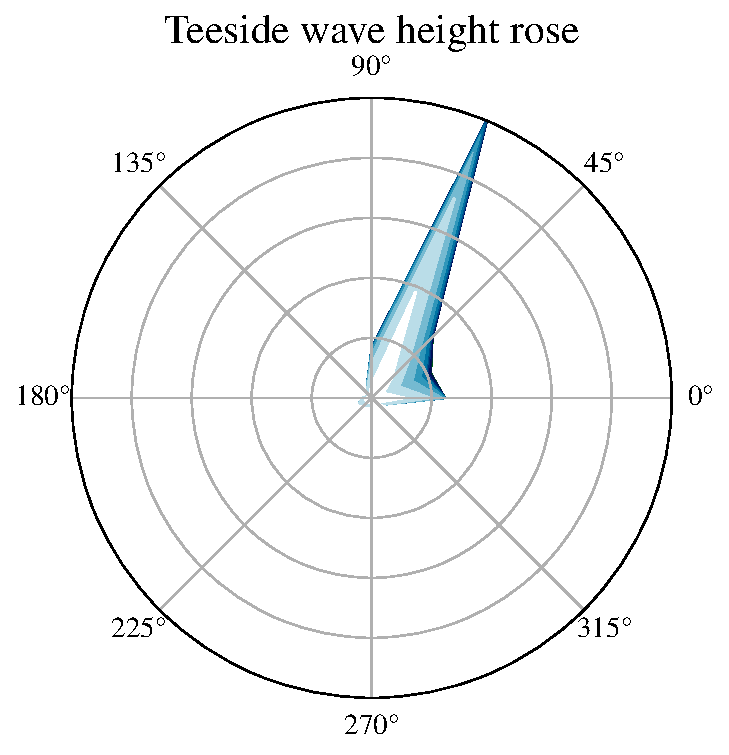
\includegraphics[width=0.3\textwidth]{part2/figures/DCE/teesside/teeside_wave_rose.pdf} \quad
    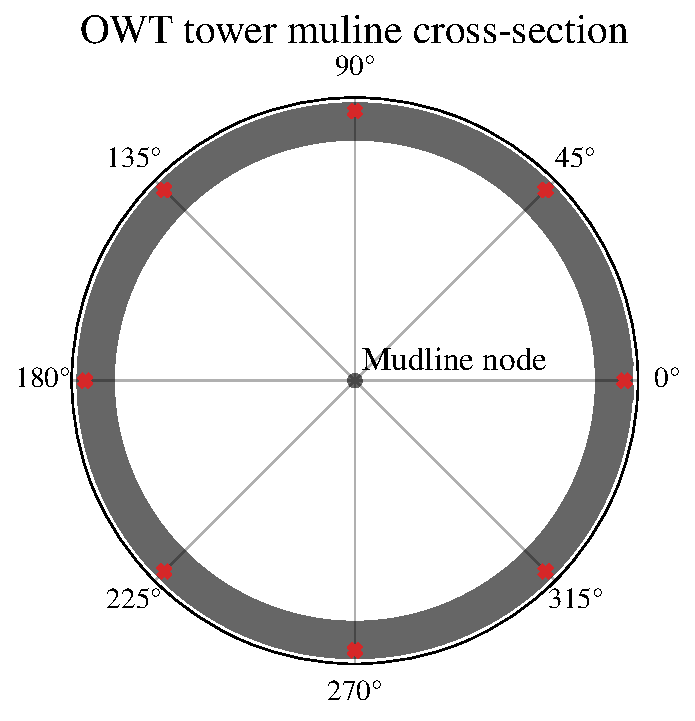
\includegraphics[width=0.3\textwidth]{part2/figures/DCE/teesside/mudline_crossection.pdf}
\end{center}
\caption{Angular distribution of the wind and waves with a horizontal cross-section of the OWT structure and the mudline\label{fig:wind_wave_roses}}
\end{figure}

\begin{figure}[!h]
\begin{center}
    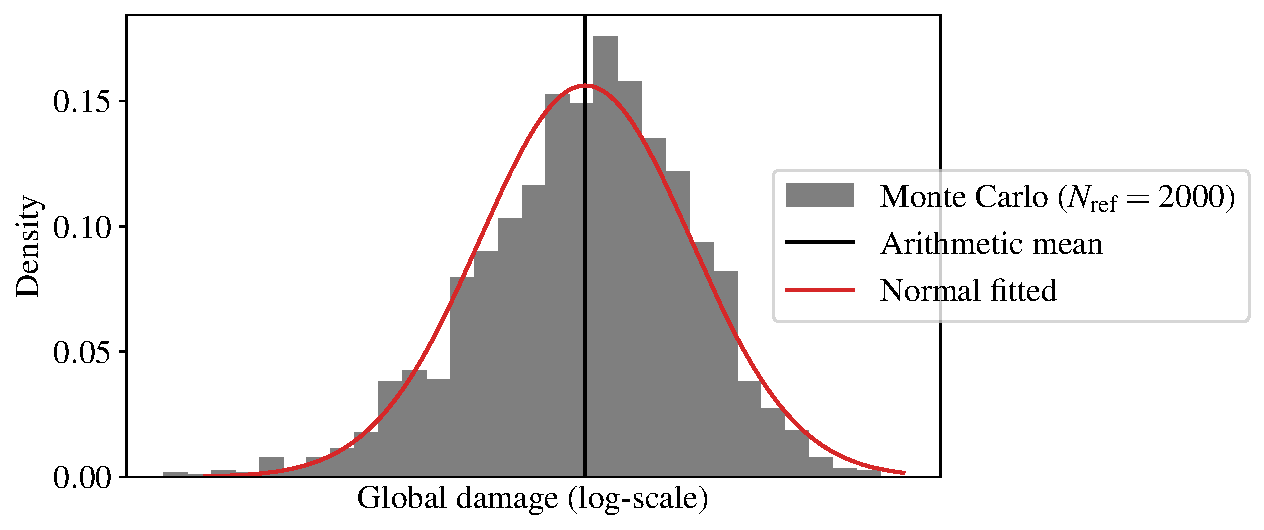
\includegraphics[width=0.7\textwidth]{part2/figures/DCE/teesside/reference_log_histogramNode1_45.pdf}
\end{center}
\caption{Histogram of the log-damage, at mudline, azimuth 45 deg. (Monte Carlo reference sample)\label{fig:histo_mc}}
\end{figure}

%============================================================%
\section{Numerical integration procedures for mean damage estimation}\label{sec3}
%============================================================%
%------------------------------------------------------------%
\subsection{Quadrature rules and quasi-Monte Carlo methods}
%------------------------------------------------------------%
The present section explores different methods aiming at estimating the expected value of a function against a probability measure. 
Considering a measurable space $\iD_\bX \subset \R^p, p \in \N_+$, associated with a known Lebesgue measure $\mu$, let us study the approximation of integrals of the form $\int_{\iD_\bX} g(\bx) \dd\mu(\bx)$, with $g$ the map $g(\bx): \iD_\bX \to \R$. 
This problem is equivalent to the central tendency estimation of $\bY = g(\bX)$, the image of the environmental random variable $\bX$ by the damage function $g$ (see \eq{eq:mean_integral}). 
Some authors also named this generic problem \emph{probabilistic integration} \citep{briol_oates_2019}. 
In practice, this quantity of interest is estimated on an $n$-sized set of damage realizations $\by_n = \left\{g(\bx^{(1)}), \dots, g(\bx^{(n)})\right\}$ of an input sample $\bX_n = \left\{\bx^{(1)}, \dots, \bx^{(n)}\right\}$. 
Our numerical experiment framework often implies that the function $g$ is costly to evaluate, making the realization number limited. 
A weighted arithmetic mean of the realizations $\left\{g(\bx^{(1)}), \dots, g(\bx^{(n)})\right\}$ is called a \emph{quadrature rule} with a set of unconstrained weights $\bw_n = \{w_1, \dots, w_n\} \in \R^n$:
\begin{equation}
    I_{\mu}(g) := \int_{\iD_\bX} g(\bx) \dd\mu(\bx) \approx \sum_{i=1}^n w_i g(\bx^{(i)}).
    \label{eq:quadrature_rule}
\end{equation}
For a given sample size $n$, our goal is to find a set of tuples $\left\{\bx^{(i)}, w_i \right\}_{i=1}^n$ (i.e., quadrature rule), giving the best approximation of our quantity. 
In the literature, a large panel of numerical integration methods has been proposed to tackle this problem. 
In a recent work, \cite{bos_2020} applies a first family of numerical integration methods based on tensor products of quadrature rules to a similar industrial OWT use case. 
Unfortunately, the tensor formulation fails when inputs present a strong dependency structure and will not be studied in this paper. 
Alternatively, sampling methods rely on generating a set of points $\bX_n$ drawn from the input distribution to compute the arithmetic mean of their realizations (i.e., uniform weights $\left\{w_i = \frac1n \right\}_{i=1}^n$). 
Among them, low-discrepancy sequences, also called ``quasi-Monte Carlo'' sampling (e.g., Sobol', Halton, Faure sequences) are known to improve the standard Monte Carlo convergence rate and will be used as a deterministic reference method in the following numerical experiments \citep{morokoff_1995}.

%------------------------------------------------------------%
\subsection{Kernel discrepancy}
%------------------------------------------------------------%
\paragraph{Quantization of probability measures and quadrature}
%------------------------------------------------------------%
When dealing with probabilistic integration such as \eq{eq:quadrature_rule}, a quadrature rule is a finite representation of a continuous measure $\mu$ by a discrete measure $\zeta_n = \sum_{i=1}^n w_i \delta(\bx^{(i)})$ (weighted sum of Dirac distributions at the design points $\bX_n$). 
In the literature, this procedure is also called \emph{quantization} of a continuous measure $\mu$. 
Overall, numerical integration is a particular case of probabilistic integration against a uniform input measure. 
For uniform measures, the Koksma-Hlawka inequality \citep{morokoff_1995} provides a useful upper bound on the absolute error of a quadrature rule: 
\begin{equation}
    \left| \int_{[0, 1]^p} g(\bx) \ddx - \frac1n \sum_{i=1}^n g(\bx^{(i)})\right| \leq  V(g) D_n^*(\bX_n).
    \label{eq:KH_inequality}
\end{equation}
As explained in \cite{oates_21}, $V(g) = \sum_{\mathfrak{u}\subseteq\{1, \dots, p \}} \int_{[0, 1]^\mathfrak{u}} \left| \frac{\partial^{\mathfrak{u}}g}{\partial \bx_{\mathfrak{u}}}(\bx_{\mathfrak{u}}, 1)\right| \dd\bx$, quantifies the complexity of the integrand, while $D_n^*(\bX_n)$ evaluates the discrepancy to uniformity of the design $\bX_n$. 
Therefore, the Koksma-Hlawka inequality shows that the quadrature rule's accuracy relies on the good quantization of $\mu$ by $\bX_n$. For a uniform target measure $\mu$, the star discrepancy is a metric assessing how far from uniformity a sample $\bX_n$ is. 
When generalizing to a non-uniform measure, a good quantization of $\mu$ should also lead to a good approximation of the quantity. %In the following, a kernel-based distance between multivariate distributions will be introduced to assess the quantization quality.

\paragraph{Reproducing kernel Hilbert space and kernel mean embedding}
%------------------------------------------------------------%
To generalize the Koksma-Hlawka inequality to any probability measure, let us assume that the integrand $g$ lives in a specific function space $\iH(k)$. $\iH(k)$ is a \emph{reproducing kernel Hilbert space} (RKHS), which is an inner product space $\iH(k)$ of functions $g:\iD_{\bX} \rightarrow \R$. 
Considering a symmetric and positive definite function $k: \iD_{\bX} \times \iD_{\bX} \rightarrow \R$, later called a ``reproducing kernel'' or simply a ``kernel'', an RKHS verifies the following axioms: 
\begin{itemize}
    \item The ``feature map'' $\phi : \iD_{\bX} \to \iH(k); \phi(\bx) = k(\cdot, \bx)$ belongs to the RKHS: $k(\cdot, \bx) \in \iH(k), \forall \bx \in \iD_{\bX}$.
    \item The ``reproducing property'': $\langle g, k(\cdot, \bx) \rangle_{\iH(k)} = g(\bx), \quad \forall \bx \in \iD_{\bX}, \forall g \in \iH(k)$.
\end{itemize}
Note that it can be shown that every positive semi-definite kernel defines a unique RKHS (and vice versa) with a feature map $\phi$, such that $k(\bx, \bx') = \langle \phi(\bx), \phi(\bx') \rangle_{\iH(k)}$.
This framework allows us to embed a continuous or discrete probability measure in an RKHS, as illustrated in \fig{fig:kernel_mean_embedding}. 
For any measure $\mu$, its \emph{kernel mean embedding} \citep{sejdinovic_2013}, also called ``potential'' $P_{\mu}(\bx)$ in \cite{pronzato_zhigljavsky_2020}, associated with the kernel $k$ is defined as:

\begin{equation}
   P_{\mu}(\bx) := \int_{\iD_{\bX}} k(\bx, \bx') \dd \mu(\bx').
\end{equation}

Respectively, the potential $P_{\zeta_n}(\bx)$ of a discrete distribution $\zeta_n = \sum_{i=1}^{n} w_i \delta(\bx^{(i)}), w_i \in \R$ associated with the kernel $k$ can be written as:
\begin{equation}\label{eq:potential}
    %P_{\mu}(\bx) := \int_{\iD_{\bX}} k(\bx, \bx') \d \mu(\bx'), \qquad 
    P_{\zeta_n}(\bx) =  \int_{\iD_{\bX}} k(\bx, \bx') \dd \zeta_n(\bx') = \sum_{i=1}^{n} w_i k(\bx, \bx^{(i)}).
\end{equation}
The potential $P_{\mu}(\bx)$ of the targeted measure $\mu$ will be referred to as ``target potential'' and the potential $P_{\zeta_n}(\bx)$ associated with the discrete distribution $\zeta_n$ called ``current potential'' when its support is the design $\bX_n$. 
If $P_{\zeta_n}(\bx)$ is close to $P_{\mu}(\bx)$, it can be interpreted to mean that $\zeta_n$ is an adequate quantization or representation of $\mu$ by the discrete distribution $\zeta_n$ (and therefore lead to a good estimation of a quantity such as $I_{\mu}(g)$ from \eq{eq:quadrature_rule}). 
Potentials can be computed in closed forms for specific pairs of distribution and associated kernel. 
Summary tables of some of these cases are detailed in \cite{briol_phd_2019} (section 3.4), \cite{pronzato_zhigljavsky_2020} (section 4), and extended in \cite{fekhari_iooss_2023}. 
However, in most cases, the target potentials must be estimated on a large and representative sample, typically a large quasi-Monte Carlo sample of $\mu$.

\medskip
\begin{definition}
The \emph{energy} of a measure $\mu$ is defined as the integral of the potential $P_\mu$ against the measure, which leads to the following scalar quantity:
\begin{equation}
    \varepsilon_\mu:= \int_{\iD_{\bX}} P_{\mu}(\bx) \dd \mu(\bx) = \iint_{\iD_{\bX}^2} k(\bx, \bx')\, \dd\mu(\bx) \dd\mu(\bx').
\end{equation}
\label{eq:target_energy}
\end{definition}

\begin{figure}[!h]
    \centering
    \begin{tikzpicture}[thick, scale=0.7, every node/.style={transform shape}]
    % Axes
    \def\x{6}\def\y{3.5}
    \draw[-] (-0.5,0) -- (\x+0.5,0) node[right] {};
    \draw[-] (0,-0.5) -- (0,\y+0.5);

    \node (A) at (1.5, 3) {};
    \node (B) at (3.5, 1) {};
    \node (C) at ($(A)!0.5!(B)$) {};
    \draw[{|-|}, very thick] (A) -- (B);

    \fill [red!80] (A) circle (2pt) node[above, black] {$P_{\pi}$};
    \fill [red!80] (B) circle (2pt) node[below, black] {$P_{\zeta}$};
    \node (MMD) at (4.5, 3.5) {$\left\lVert P_{\pi} - P_{\zeta}\right\lVert_{\iH(k)}$};
    \draw[-stealth] (MMD) to [bend left] (C);

    \node [inner sep=0pt] (disc) at (-2,0.9) {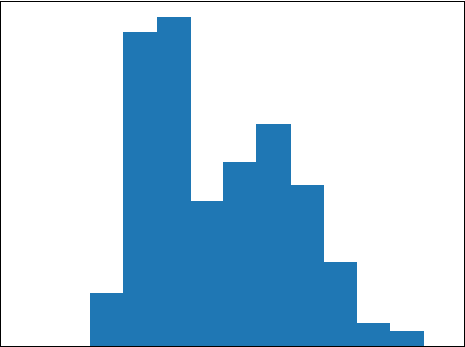
\includegraphics[width=.2\textwidth]{part2/figures/DCE/discrete.pdf}};
    \node [inner sep=0pt] (cont) at (-2,3.1) {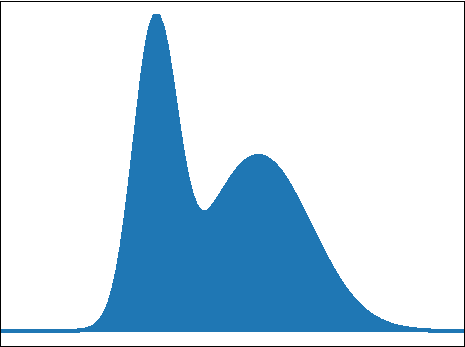
\includegraphics[width=.2\textwidth]{part2/figures/DCE/continuous.pdf}};
    \draw[-stealth] (cont) to [bend left] (A);
    \draw[-stealth] (disc.east) to [bend right] (B);
    % Text
    \node at (5, 0.25) {$\mathcal{H}_k$};
    \node at (-3, 3) {$\pi$};
    \node at (-3, 1) {$\zeta$};
\end{tikzpicture}
    \caption{Kernel mean embedding of a continuous and discrete probability distribution}
    \label{fig:kernel_mean_embedding}
\end{figure}
Finally, using the reproducing property and writing the Cauchy-Schwarz inequality on the absolute quadrature error leads to the following inequality, similar to the Koksma-Hlawka inequality \eq{eq:KH_inequality} (see \cite{briol_oates_2019}): 

\begin{subequations}
\begin{align}
    \left| \sum_{i=1}^{n} w_i g(\bx^{(i)}) - \int_{\iD_{\bX}} g(\bx) \dd \mu(\bx) \right| &= \left| \left\langle g, P_{\zeta_n}(\bx) \right\rangle_{\iH(k)} - \left\langle g, P_{\mu}(\bx) \right\rangle_{\iH(k)} \right| \\
    &= \left| \left\langle g, \left(P_{\zeta_n}(\bx) - P_{\mu}(\bx)\right) \right\rangle_{\iH(k)} \right|\\
    &\leq \lVert g \lVert_{\iH(k)}  \left\lVert P_{\mu}(\bx) - P_{\zeta_n}(\bx) \right\lVert_{\iH(k)}.
    \label{eq:quad_error}
\end{align}
\end{subequations}

\paragraph{Maximum mean discrepancy}
%------------------------------------------------------------%
A metric of discrepancy and quadrature error is offered by the \emph{maximum mean discrepancy} (MMD). 
This distance between two probability distributions $\mu$ and $\zeta$ is given by the worst-case error for any function within a unit ball of the Hilbert space $\iH(k)$, associated with the kernel $k$:
\begin{equation}
    \MMD_k(\mu, \zeta) := %\\ 
    \sup_{\lVert g \lVert_{\iH(k)} \leq 1}
            \left | \int_{\iD_{\bX}} g(\bx) \dd \mu(\bx) - \int_{\iD_{\bX}} g(\bx) \dd \zeta(\bx) \right| %= \left\lVert P_{\mu}(\bx) - P_{\zeta}(\bx) \right\lVert_{\iH(k)}.
    \label{eq:mmd}  
\end{equation}

According to the inequality in \eq{eq:quad_error}, $\MMD_k(\mu, \zeta) = \left\lVert P_{\mu} - P_{\zeta} \right\lVert_{\iH(k)}$, meaning that the MMD fully relies on the difference of potentials. 
Moreover, \cite{sriperumbudur_2010} defines a kernel as ``characteristic kernel'' when the following equivalence is true: $\MMD_k(\mu, \zeta) = 0 \Leftrightarrow \mu = \zeta$. 
This property makes the MMD a metric on $\iD_{\bX}$. 
The squared MMD has been used for other purposes than numerical integration: e.g., statistical testing \citep{gretton_2006}, and global sensitivity analysis \citep{daveiga_2015}. 
It can be written as follows:

\begin{subequations}
\begin{align}\label{eq:mmd2}
    \MMD_k(\mu, \zeta)^2 &= \left\lVert P_{\mu}(\bx) - P_{\zeta}(\bx) \right\lVert^2_{\iH(k)}\\
        &= \left\langle \left(P_{\mu}(\bx) - P_{\zeta}(\bx) \right), \left(P_{\mu}(\bx) - P_{\zeta}(\bx) \right) \right\rangle_{\iH(k)}\\
        &= \left\langle P_{\mu}(\bx), P_{\mu}(\bx) \right\rangle_{\iH(k)} - 2 \left\langle P_{\mu}(\bx), P_{\zeta}(\bx) \right\rangle_{\iH(k)} + \left\langle P_{\zeta}(\bx), P_{\zeta}(\bx) \right\rangle_{\iH(k)}\\
        &= \iint_{\iD_{\bX}^2} k(\bx, \bx')\, \dd\mu(\bx) \dd\mu(\bx') - 2 \iint_{\iD_{\bX}^2} k(\bx, \bx')\, \dd\mu(\bx) \dd\zeta(\bx') + \iint_{\iD_{\bX}^2} k(\bx, \bx')\, \dd\zeta(\bx) \dd\zeta(\bx').
\end{align}
\end{subequations}
Taking a discrete distribution with uniform weights $\zeta_n= \frac{1}{n} \sum_{i=1}^{n} \delta(\bx^{(i)})$, the squared MMD reduces to: 
\begin{equation}\label{eq:mmd_design}
    \MMD_k(\mu, \zeta_n)^2 = \varepsilon_\mu - \frac{2}{n} \sum_{i=1}^n P_{\mu}\left(\bx^{(i)}\right) + \frac{1}{n^2} \sum_{i, j=1}^n k\left(\bx^{(i)}, \bx^{(j)}\right).
\end{equation}
%\begin{remark}
% Should we compare MMD to other divergences (see Sriperumbudur 2010)?
%A strong link exists between numerical integration and space-filling design of experiments. The MMD yields an upper bound over a geometric space-filling metric called the ``covering radius'' (see section 4.1.2 in \cite{pronzato_zhigljavsky_2020}). 
%\end{remark}

%------------------------------------------------------------%
\subsection{Kernel herding sampling}\label{sec:khsubsec}
%------------------------------------------------------------%
Herein, the MMD is used to quantize the known target measure $\mu$ by a design sample $\bX_n$. 
For practical reasons, design construction is done sequentially. 
Sequential strategies can also be used to learn and validate regression models for statistical learning (see \cite{fekhari_iooss_2023}). 
Moreover, since each realization is supposed to be obtained at the same unitary cost, we fix the quadrature weights as uniform during the construction of the design $\bX_n$.

\emph{Kernel herding} (KH), proposed by \cite{chen_welling_2010}, is a sampling method that offers a quantization of the measure $\mu$ by minimizing a squared MMD when adding points iteratively. 
With a current design $\bX_n$ and its corresponding discrete distribution with uniform weights $\zeta_n= \frac{1}{n} \sum_{i=1}^{n} \delta(\bx^{(i)})$, a KH iteration can be written as an optimization problem involving the following criterion over the point $\bx^{(n+1)} \in \iD_{\bX}$:
\begin{align}
   \bx^{(n+1)} \in \argmin_{\bx \in \iD_{\bX}} \left\{\MMD_k\left(\mu, \frac{1}{n+1} \left(\delta(\bx) + \sum_{i=1}^{n} \delta(\bx^{(i)})\right)\right)^2\right\}.
   % = \argmin_{\bx \in \iD_{\bX}} \MMD_k\left(\mu, \frac{1}{n+1} \left(n \zeta_n  + \delta(\bx)\right)\right)
   \label{eq:mmd_criterion}
\end{align}

In the literature, two formulations of this optimization problem can be found. 
The first one uses the Frank-Wolfe algorithm (or ``conditional gradient algorithm'') to compute a linearization of the problem under the convexity hypothesis (see \cite{lacoste_2015} and \cite{briol_2015} for more details). 
The second one is a straightforward greedy optimization. Due to the combinatorial complexity, the greedy formulation is tractable for sequential construction. 
To see this, let us develop the MMD from \eq{eq:mmd_design}:
\begin{subequations}
\begin{align}
    \MMD_k\left(\mu, \frac{1}{n+1} \left(\delta(\bx) + \sum_{i=1}^{n} \delta(\bx^{(i)})\right)\right)^2
    &= \varepsilon_\mu - \frac{2}{n+1} \sum_{i=1}^{n+1} P_{\mu}\left(\bx^{(i)}\right) + \frac{1}{(n+1)^2} \sum_{i,j=1}^{n+1} k\left(\bx^{(i)}, \bx^{(j)}\right)\\
    &= \varepsilon_\mu - \frac{2}{n+1} \left(P_\mu(\bx) + \sum_{i=1}^n P_{\mu}\left(\bx^{(i)}\right)\right)\\ &+ \frac{1}{(n+1)^2} \left(\sum_{i,j=1}^n k\left(\bx^{(i)}, \bx^{(j)}\right) + 2\sum_{i=1}^n k\left(\bx^{(i)}, \bx\right) - k(\bx, \bx) \right).
\end{align}
\end{subequations}
In the previously developed expression, only a few terms actually depend on the next optimal point $\bx^{(n+1)}$ since the target energy, denoted by $\varepsilon_\mu$, and $k(\bx, \bx)=\sigma^2$ are constant (by taking a stationary kernel). 
Therefore, the greedy minimization of the MMD can be equivalently written as: 
\begin{equation}\label{eq:greedy_formulation}
    \bx^{(n+1)} \in \argmin_{\bx \in \iD_{\bX}} \left\{ \frac{1}{n+1} \sum_{i=1}^n k\left(\bx^{(i)}, \bx\right) - P_\mu(\bx) \right\} = \argmin_{\bx \in \iD_{\bX}} \left\{ \frac{n}{n+1} P_{\zeta_n}(\bx) - P_{\mu}(\bx)\right\}.
\end{equation}

\medskip
\begin{remark}
For the sequential and uniformly weighted case, the formulation in \eq{eq:greedy_formulation} is almost similar to the Frank-Wolfe formulation. 
Our numerical experiments showed that these two versions generate very close designs, especially as $n$ becomes large. 
\cite{pronzato_rendas_2021} express the Frank-Wolfe formulation in the sequential and uniformly weighted case as follows:
\begin{align}
   \bx^{(n+1)} \in \argmin_{\bx \in \iD_{\bX}} \left\{P_{\zeta_n}(\bx) - P_{\mu}(\bx)\right\}.
   \label{eq:kh_criterion}
\end{align}
\end{remark}
\smallskip

\begin{remark}
In practice, the optimization problem is solved by a brute-force approach on a fairly dense finite subset $\iS\subseteq\iD_{\bX}$ of candidate points with size $N \gg n$ that emulates the target distribution, also called the ``candidate set''. 
This sample is also used to estimate the target potential $P_\mu(\bx) \approx \frac1N \sum_{i=1}^N k\left(\bx^{(i)}, \bx\right)$.
\end{remark}
\medskip

As explained previously, choosing the kernel defines the function space on which the worst-case function is found (see \eq{eq:mmd}). 
Therefore, this sampling method is sensitive to kernel choice. 
A kernel is defined, both by the choice of its parametric family (e.g., Matérn, squared exponential) and the choice of its tuning. 
The so-called ``support points'' method developed by \cite{mak_joseph_2018} is a special case of kernel herding that uses the characteristic and parameter-free ``energy-distance'' kernel (introduced by \cite{szekely_rizzo_2013}). 
In the following numerical experiments, the energy-distance kernel will be compared with an isotropic tensor product of a Matérn kernel (with regularity parameter $\nu = 5/2$ and correlation lengths $\theta_i$), or a squared exponential kernel (with correlation lengths $\theta_i$) defined in Table \ref{tab:kernels}. 
Since the Matérn and squared exponential kernels are widely used for Gaussian process regression \citep{rasmussen_2006}, they were naturally picked to challenge the energy-distance kernel. 
The correlation lengths for the squared exponential and Matérn kernels are set using the heuristic given in \cite{fekhari_iooss_2023}, $\theta_i = n^{-1/p}, i \in \{1, \dots, p\}$. 

\begin{table*}[h] \caption{Kernels considered in the following numerical experiments.}
\begin{center}
%\tabletext{
\begin{tabular*}{\textwidth}{@{\extracolsep\fill}lll@{}}
\hline
Energy-distance & $k_E(\bx,\bx') = \frac12\, \left(\| \bx \| + \| \bx' \| - \| \bx-\bx' \|\right)$ & \\
Squared exponential & $k_G(\bx,\bx') = \prod_{i=1}^{p} k_{\theta_{i}}(x_{i}-x'_i)$ & $k_{\theta}(x-x') = \exp \left(- \frac{(x-x')^2}{2\theta^2}\right)$\\
Matérn $(\nu = 5/2)$ & $k_M(\bx,\bx') = \prod_{i=1}^{p} k_{5/2,\theta_{i}}(x_{i}-x'_i)$
 & $k_{5/2,\theta}(x-x') = \Bigl(1 + \frac{\sqrt{5}}{\theta} |x - x'|$ \\ 
 & & $\quad + \frac{5}{3 \theta^2} (x - x')^2 \Bigr) \exp \left( - \frac{\sqrt{5}}{\theta} |x - x'| \right)$ \\
\hline
\end{tabular*}
\label{tab:kernels}
%}
\end{center}
\end{table*}

\fig{fig:kernels} represents the covariance structure of the three kernels. 
One can notice that the squared exponential and Matérn $\nu = 5/2$ kernels are closer to one another than they are to the energy-distance. 
In fact, as $\nu$ tends to infinity, the Matérn kernel tends toward the squared exponential kernel (which has infinitely differentiable sample paths, see \cite{rasmussen_2006}). 
For these two stationary kernels, the correlation length controls how fast the correlation between two points decreases as their distance from one another increases. 
Meanwhile, the energy distance is not stationary (but still positive and semi-definite). 
Therefore, its value does not only depend on the distance between two points but also on the norm of each of the points.

\begin{figure}[!h]
\begin{center}
    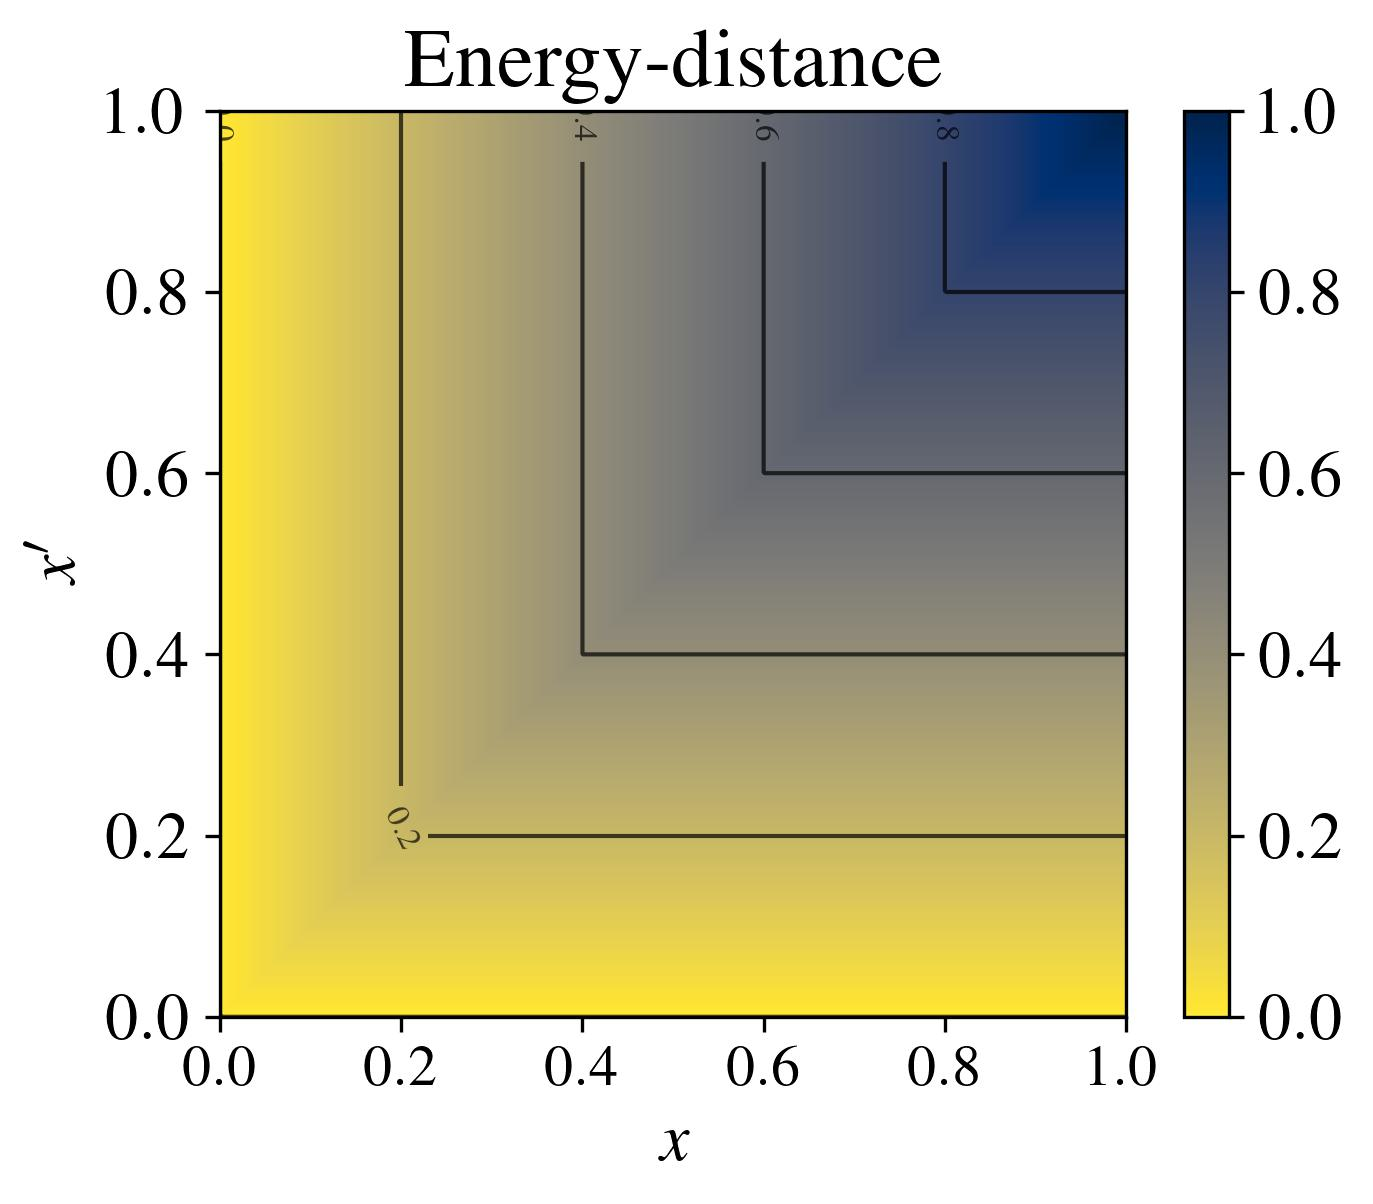
\includegraphics[width=0.32\textwidth]{part2/figures/DCE/numerical_experiments/energy_kernel.jpg}
    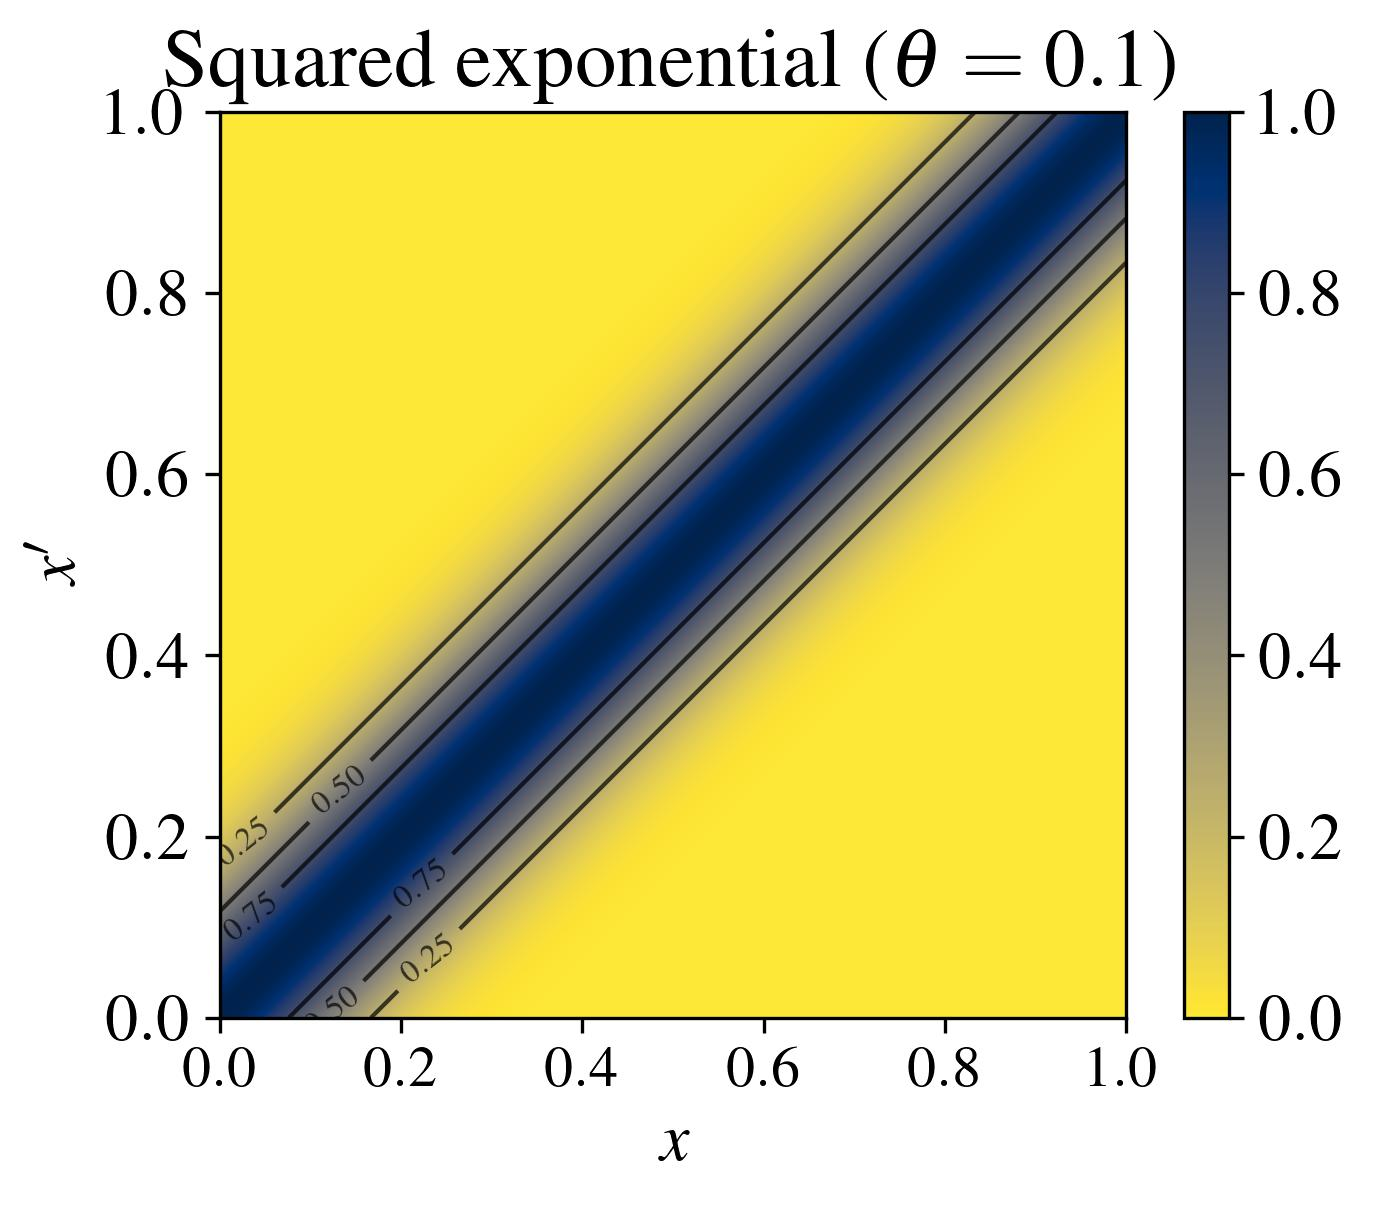
\includegraphics[width=0.32\textwidth]{part2/figures/DCE/numerical_experiments/gaussian_kernel.jpg}
    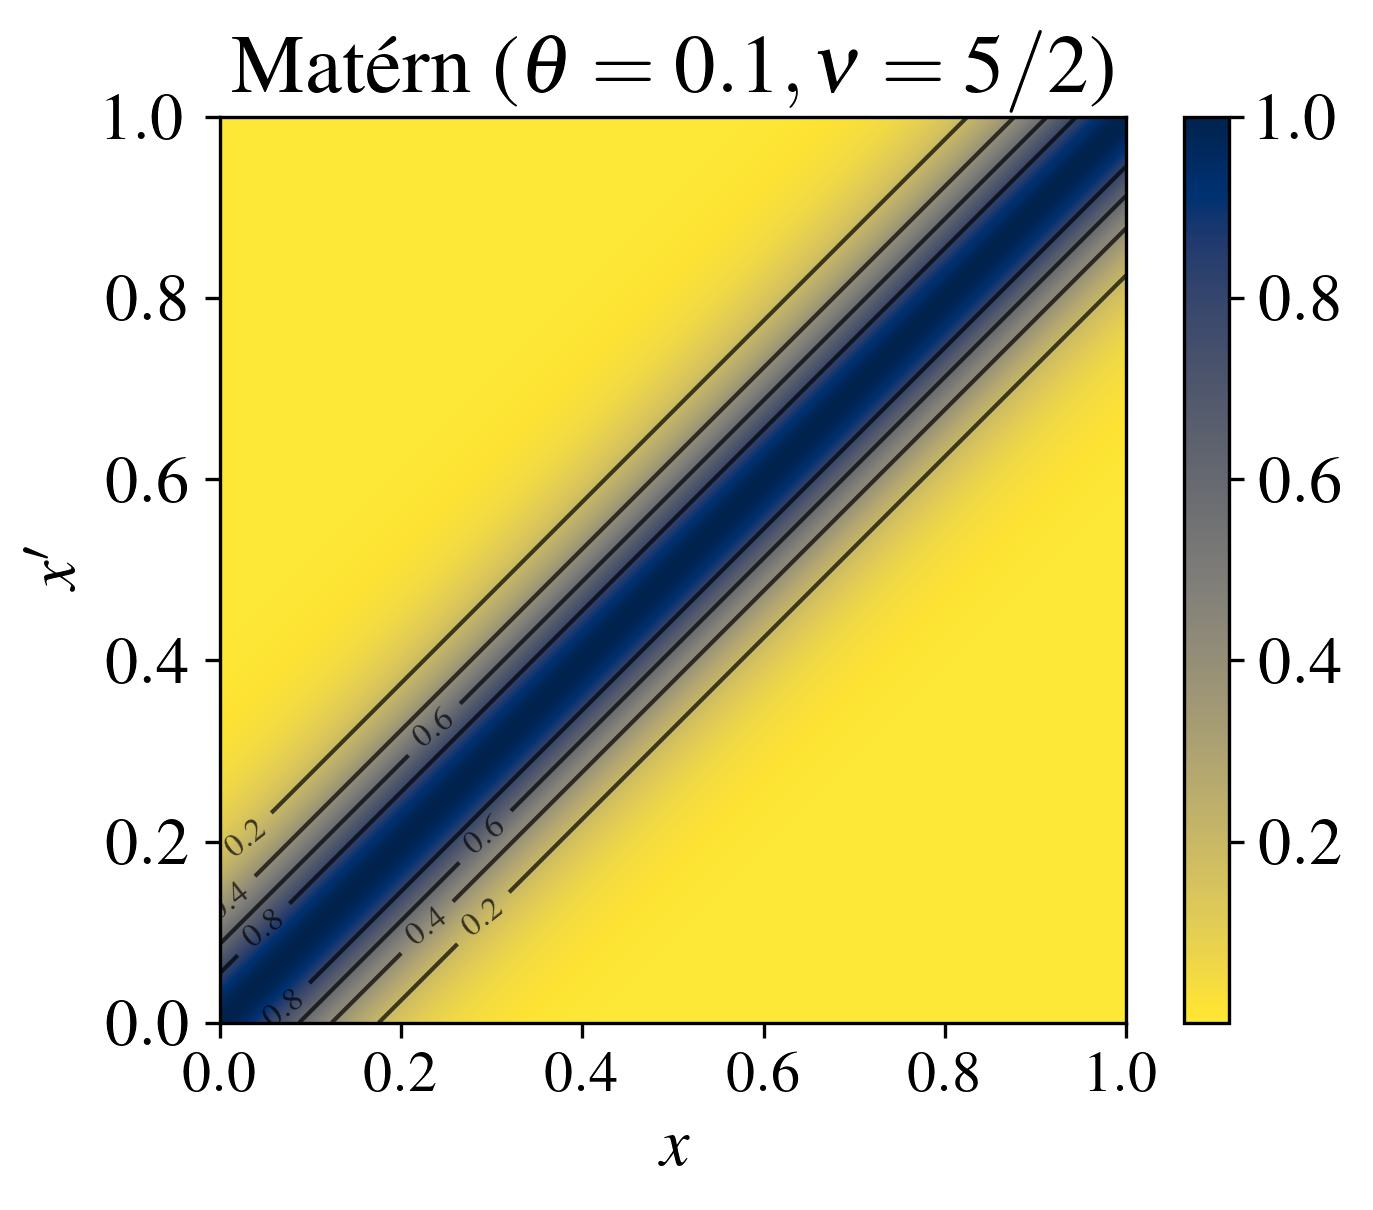
\includegraphics[width=0.32\textwidth]{part2/figures/DCE/numerical_experiments/matern_kernel.jpg}
\end{center}
\caption{Kernel illustrations (left to right: energy-distance, squared exponential, and Matérn $5/2$)} \label{fig:kernels}
\end{figure}

To illustrate the sequential sampling of a complex distribution, \fig{fig:KH_mixture} shows three nested kernel herding samples (orange crosses for different sizes $n\in\{10, 20, 40\}$) of a mixture of Gaussian distributions with complex nonlinear dependencies (with density represented by the black isoprobability contours). 
In this example, the method seems to build a parsimonious design between each mode of the distribution. 
The candidate set (in light grey) was generated by a large quasi-Monte sample of the underlying Gaussian mixture. 
In this two-dimensional case, this candidate set is sufficient to estimate the target potential $P_{\mu}$. %Since quasi-Monte Carlo sampling is subject to the curse of dimensionality, the candidate set could be generated by crude Monte Carlo for high-dimensional problems. 
However, the main bottleneck of kernel herding is the estimation of the potentials, which becomes costly in high dimension.

\begin{figure}[!h]
\begin{center}
    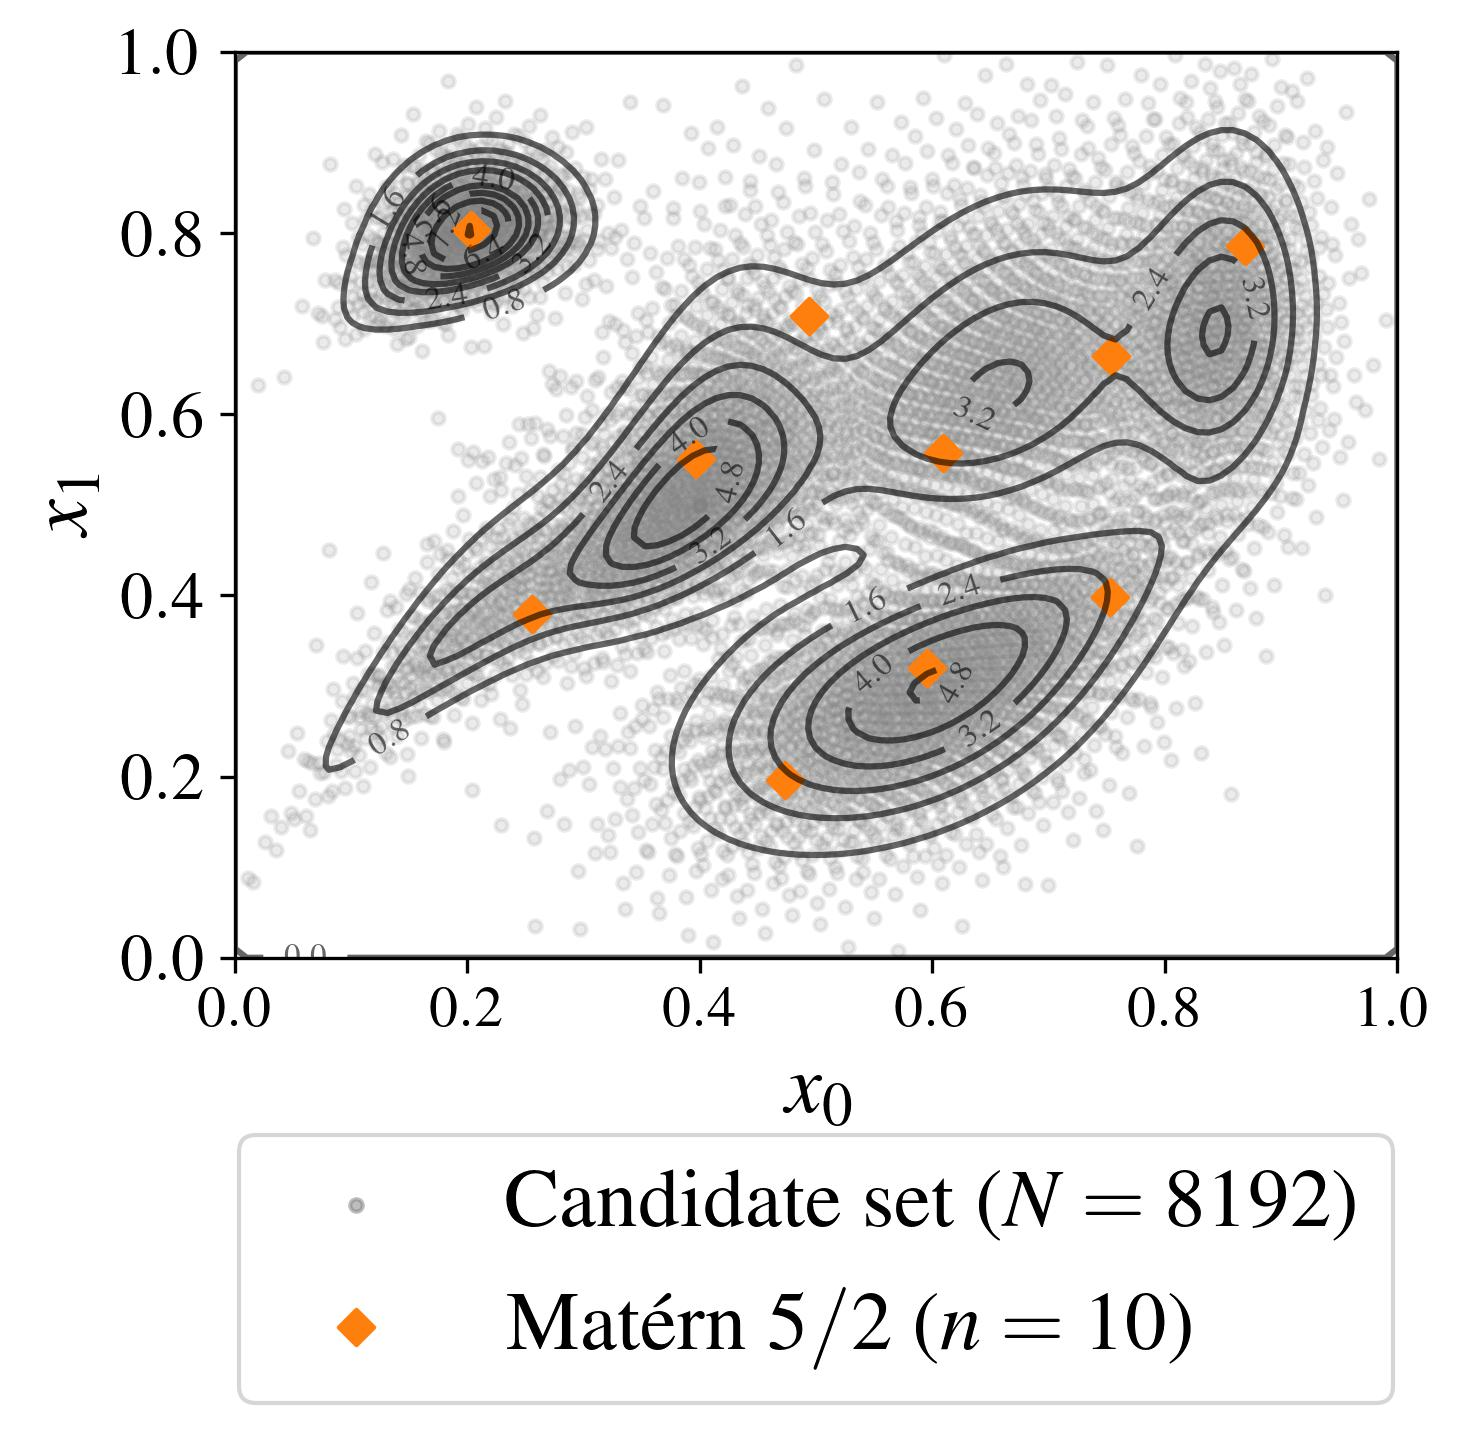
\includegraphics[width=0.32\textwidth]{part2/figures/DCE/numerical_experiments/gaussian_mixture_sampling10.jpg}
    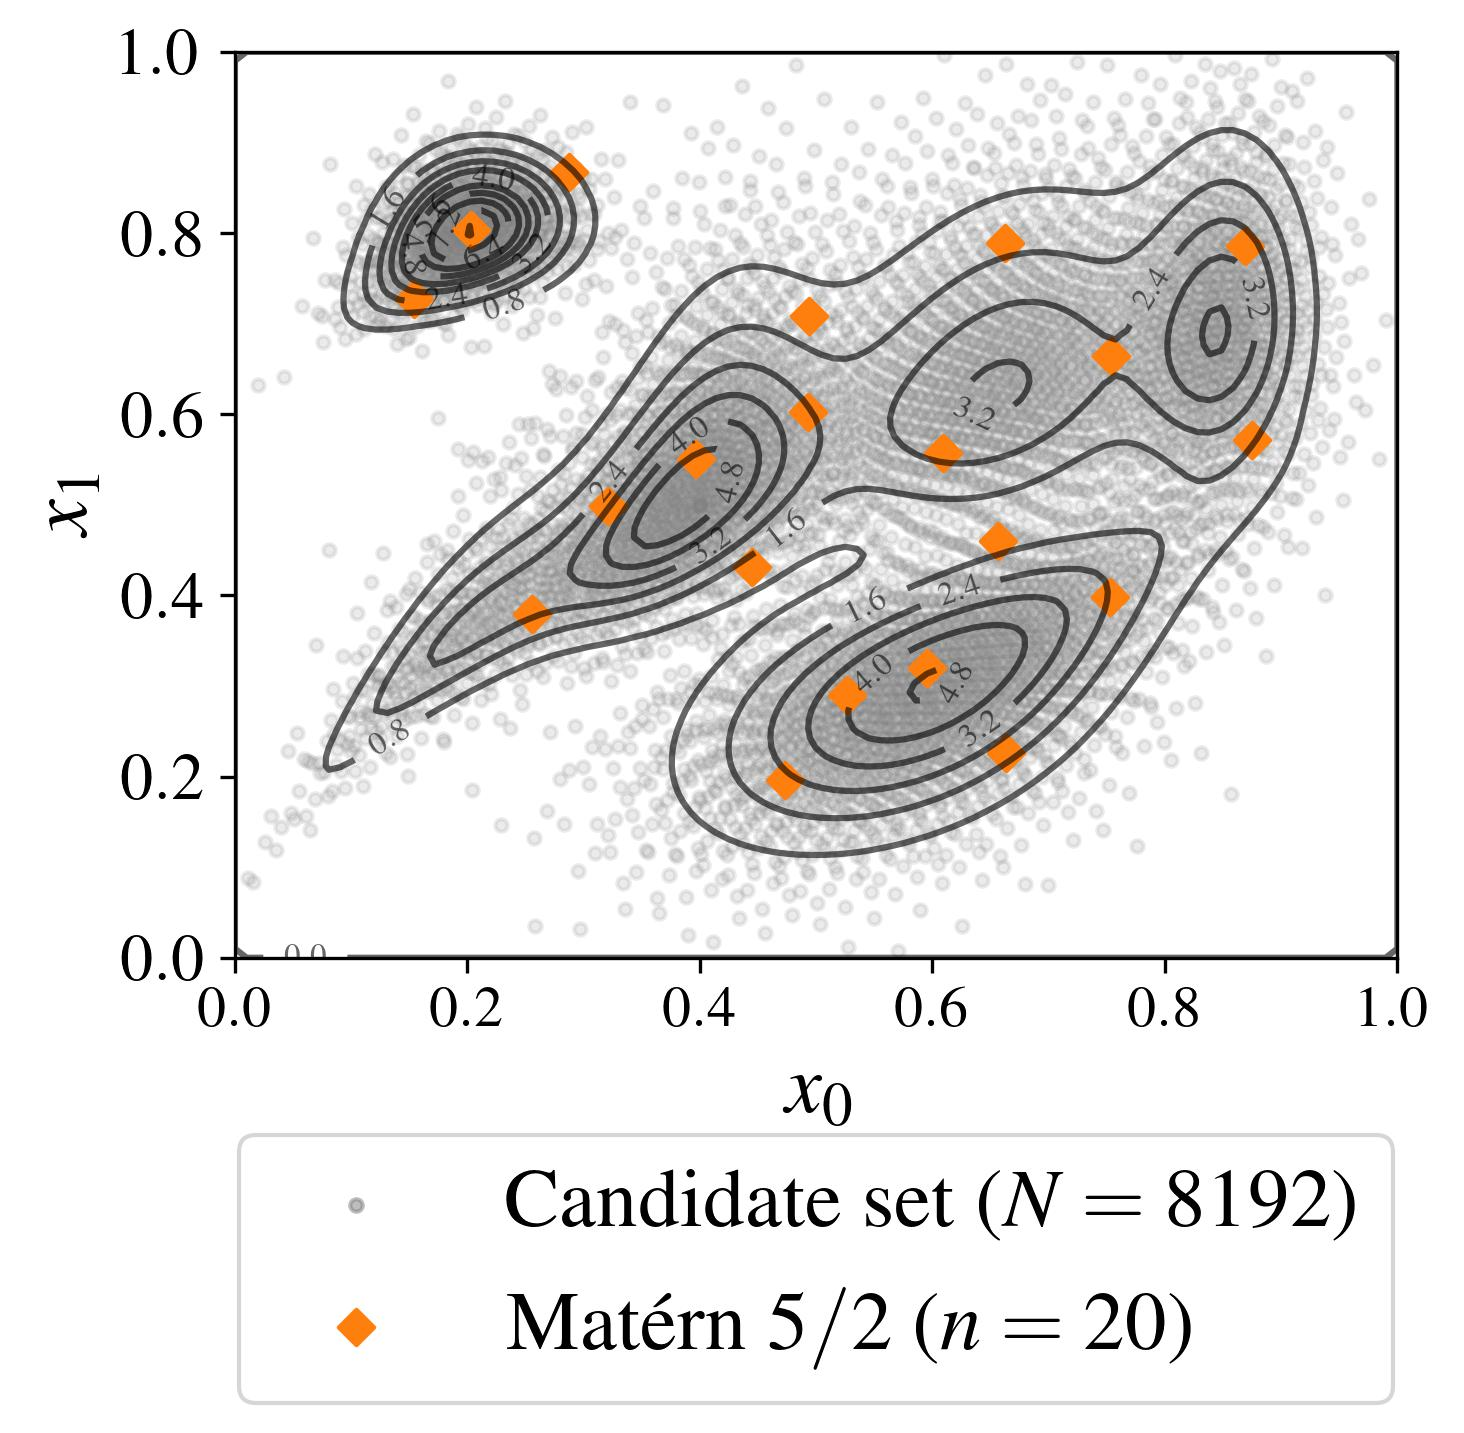
\includegraphics[width=0.32\textwidth]{part2/figures/DCE/numerical_experiments/gaussian_mixture_sampling20.jpg}
    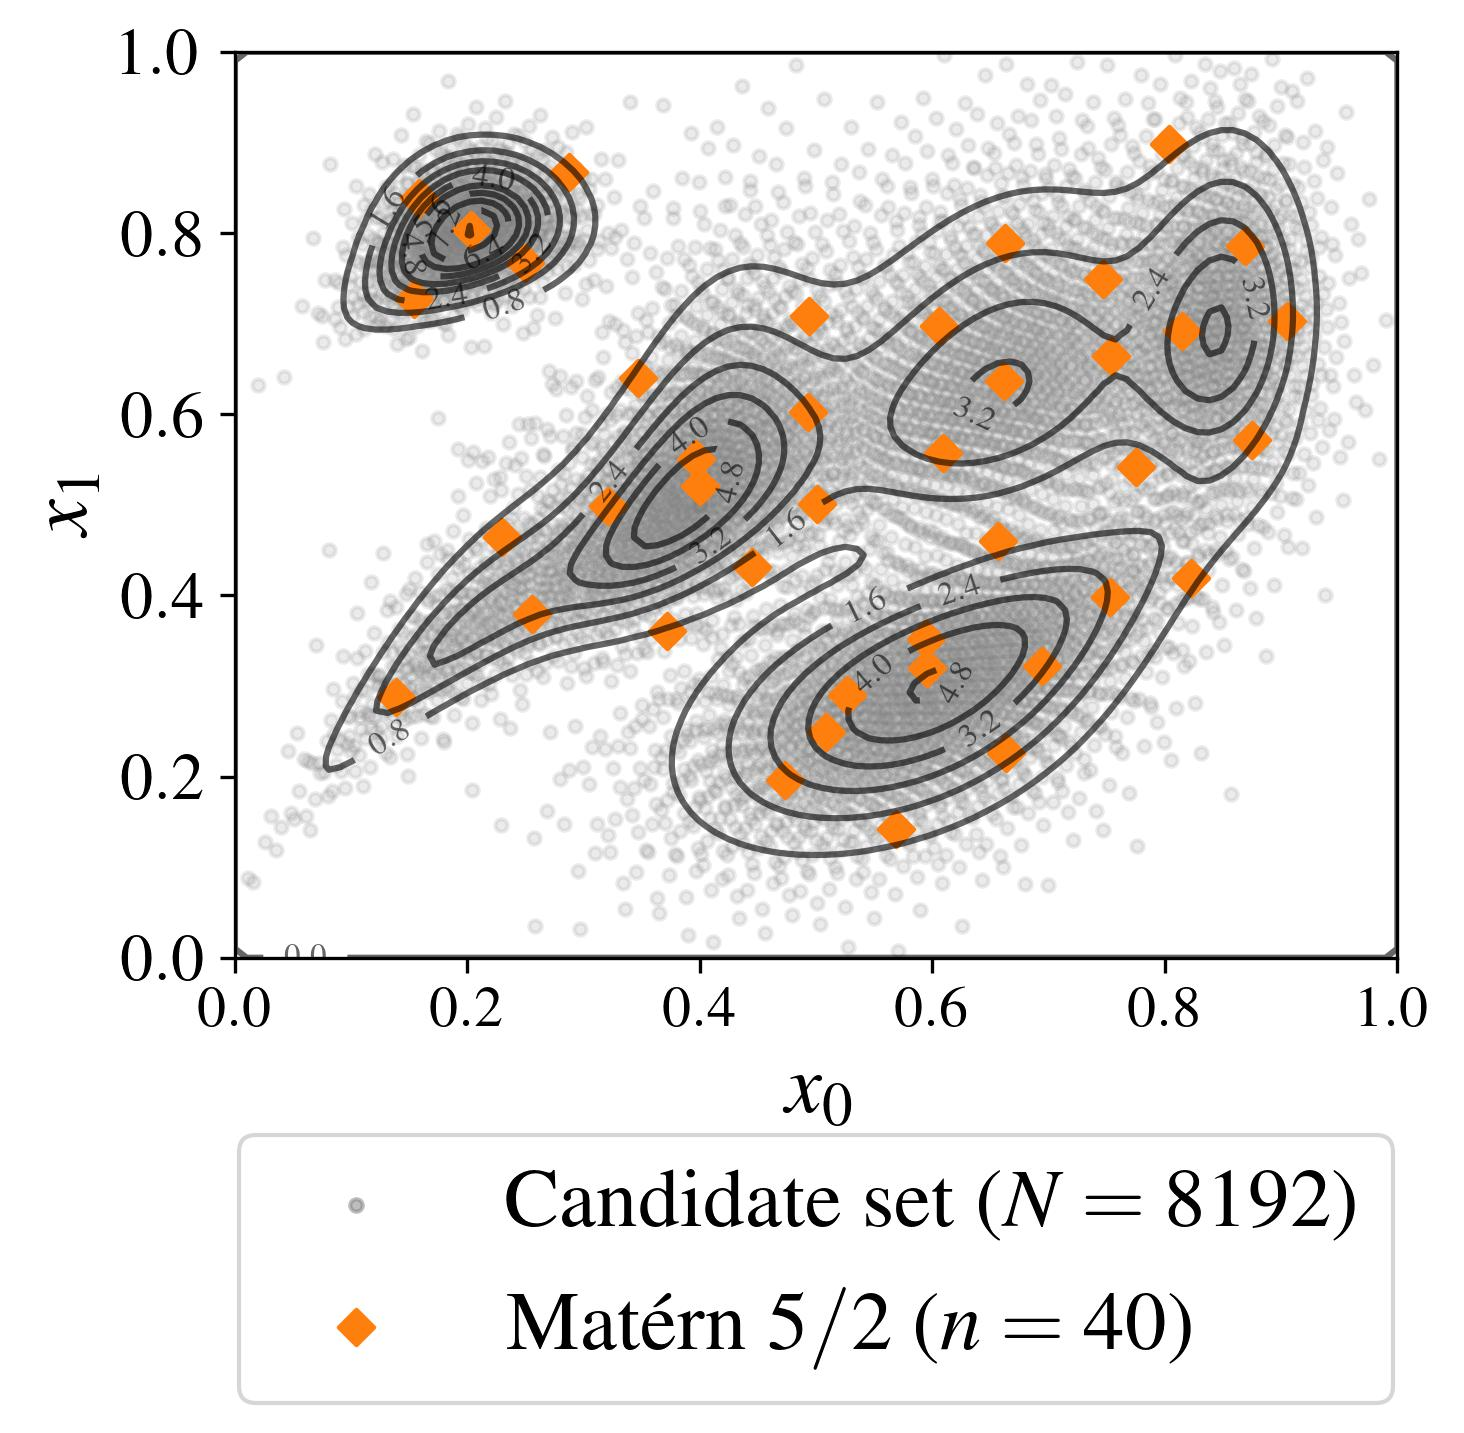
\includegraphics[width=0.32\textwidth]{part2/figures/DCE/numerical_experiments/gaussian_mixture_sampling40.jpg}
\end{center}
\caption{Sequential kernel herding for increasing design sizes ($n\in\{10, 20, 40\}$) built on a candidate set of $N=8196$ points drawn from a complex Gaussian mixture $\mu$} \label{fig:KH_mixture}
\end{figure}

%%%%%%%%%%%%%%%%%%
Other approaches take advantage of the progressive knowledge acquired sequentially on $g$ to select the following points in the design. 
These methods are sometimes called ``active learning'' or ``adaptive strategies'' \citep{fau_2021}. 
Many of them rely on a sequentially updated Gaussian process (or Kriging) metamodel. 
To solve a probabilistic integration problem, the concept of Bayesian quadrature is introduced in the following. 

%Mention KSD and Greedy Stein points? Cite \cite{teymur_gorham_2021}?

%------------------------------------------------------------%
\subsection{Bayesian quadrature}
%------------------------------------------------------------%
\paragraph{Gaussian processes for Bayesian quadrature}%------%
Kernel methods and Gaussian processes present a lot of connections and equivalences, thoroughly reviewed by \cite{motonobu_2018}. 
In numerical integration, Gaussian processes have been used to build quadrature rules in the seminal paper of \cite{ohagan_1991}, introducing the concept of \emph{Bayesian quadrature} (BQ). 
Let us recall the probabilistic integration problem $I_\mu(g) = \int_{\iD_\bX} g(\bx) \dd \mu(\bx)$ (introduced in \eq{eq:quadrature_rule}). 
From a general point of view, this quantity could be generalized by composing $g$ with another function $\psi$ (e.g., other moments, quantiles, exceedance probabilities). 
The quantity of interest then becomes, $I_\mu(\psi(g))$, for example when $\psi$ is a monomial, it gives a moment the distribution of the output.

Let us assume, adopting a Bayesian point of view, that $\xi$ is a stochastic process describing the uncertainty affecting the knowledge about the true function $g$. 
Let $\xi$ be a Gaussian process (GP) prior with a zero trend (denoted by $\textbf{0}$) to ease the calculation, and a stationary covariance kernel (denoted by $k(\cdot, \cdot)$). 
The conditional posterior $\xi_n := (\xi | \by_n) \sim \mathcal{GP}(\eta_n, s_n^2)$ has been conditioned on the function observations $\by_n = \left[g\left(\bx^{(1)}\right), \ldots, g\left(\bx^{(n)}\right)\right]\TT$ computed from the input design $\bX_n$ and is fully defined by the well-known ``Kriging equations'' (see e.g., \cite{rasmussen_2006}):
\begin{equation}
    \left\{
    \begin{array}{ll}
        \eta_n(\bx) &:= \bk_n\TT(\bx) \bK_n^{-1} \by_n\\
        s_n^2(\bx) &:= k_n(\bx, \bx) - \bk_n\TT(\bx) \bK_n^{-1} \bk_n(\bx)
    \end{array}
\right.
\label{eq:kriging}
\end{equation}
where $\bk_n(\bx)$ is the column vector of the covariance kernel evaluations $[k_n(\bx, \bx^{(1)}), \dots,\allowbreak k_n(\bx, \bx^{(n)})]$ and $\bK_n$ is the $(n \times n)$ variance-covariance matrix such that the $(i, j)$-element is $\left\{\bK_n \right\}_{i, j}=k_n(\bx^{(i)}, \bx^{(j)})$.

In BQ, the main object is the random variable $I_{\mu}(\xi_n)$. 
According to \cite{briol_oates_2019}, its distribution on $\R$ is the pushforward of $\xi_n$ through the integration operator $I_\mu(\cdot)$, sometimes called \emph{posterior distribution}: 
\begin{equation}
    I_{\mu}(\xi_n) = \int_{\iD_\bX} (\xi(\bx) | \by_n)  \dd \mu(\bx) = \int_{\iD_\bX} \xi_n(\bx)  \dd \mu(\bx) \,.
\label{eq:posterior}
\end{equation}

\fig{fig:bayesian_quad} provides a one-dimensional illustration of the Bayesian quadrature of an unknown function (dashed black curve) against a given input measure $\mu$ (with corresponding grey distribution at the bottom). 
For an arbitrary design, one can fit a Gaussian process model, interpolating the function observations (black crosses). 
Then, multiple trajectories of this conditioned Gaussian process $\xi_n$ are drawn (orange curves) whilst its mean function, also called ``predictor'', is represented by the red curve. 
Therefore, the input measure $\mu$ is propagated through the conditioned Gaussian process to obtain the random variable $I_{\mu}(\xi_n)$, with distribution represented on the right plot (brown curve). 
Again on the right plot, remark how the mean of this posterior distribution (brown line) is closer to the reference output expected value (dashed black line) than the arithmetic mean of the observations (black line). 
This plot was inspired by the paper of \cite{husar_duvenaud_2012}.

\begin{figure}[!h]
\begin{center}
    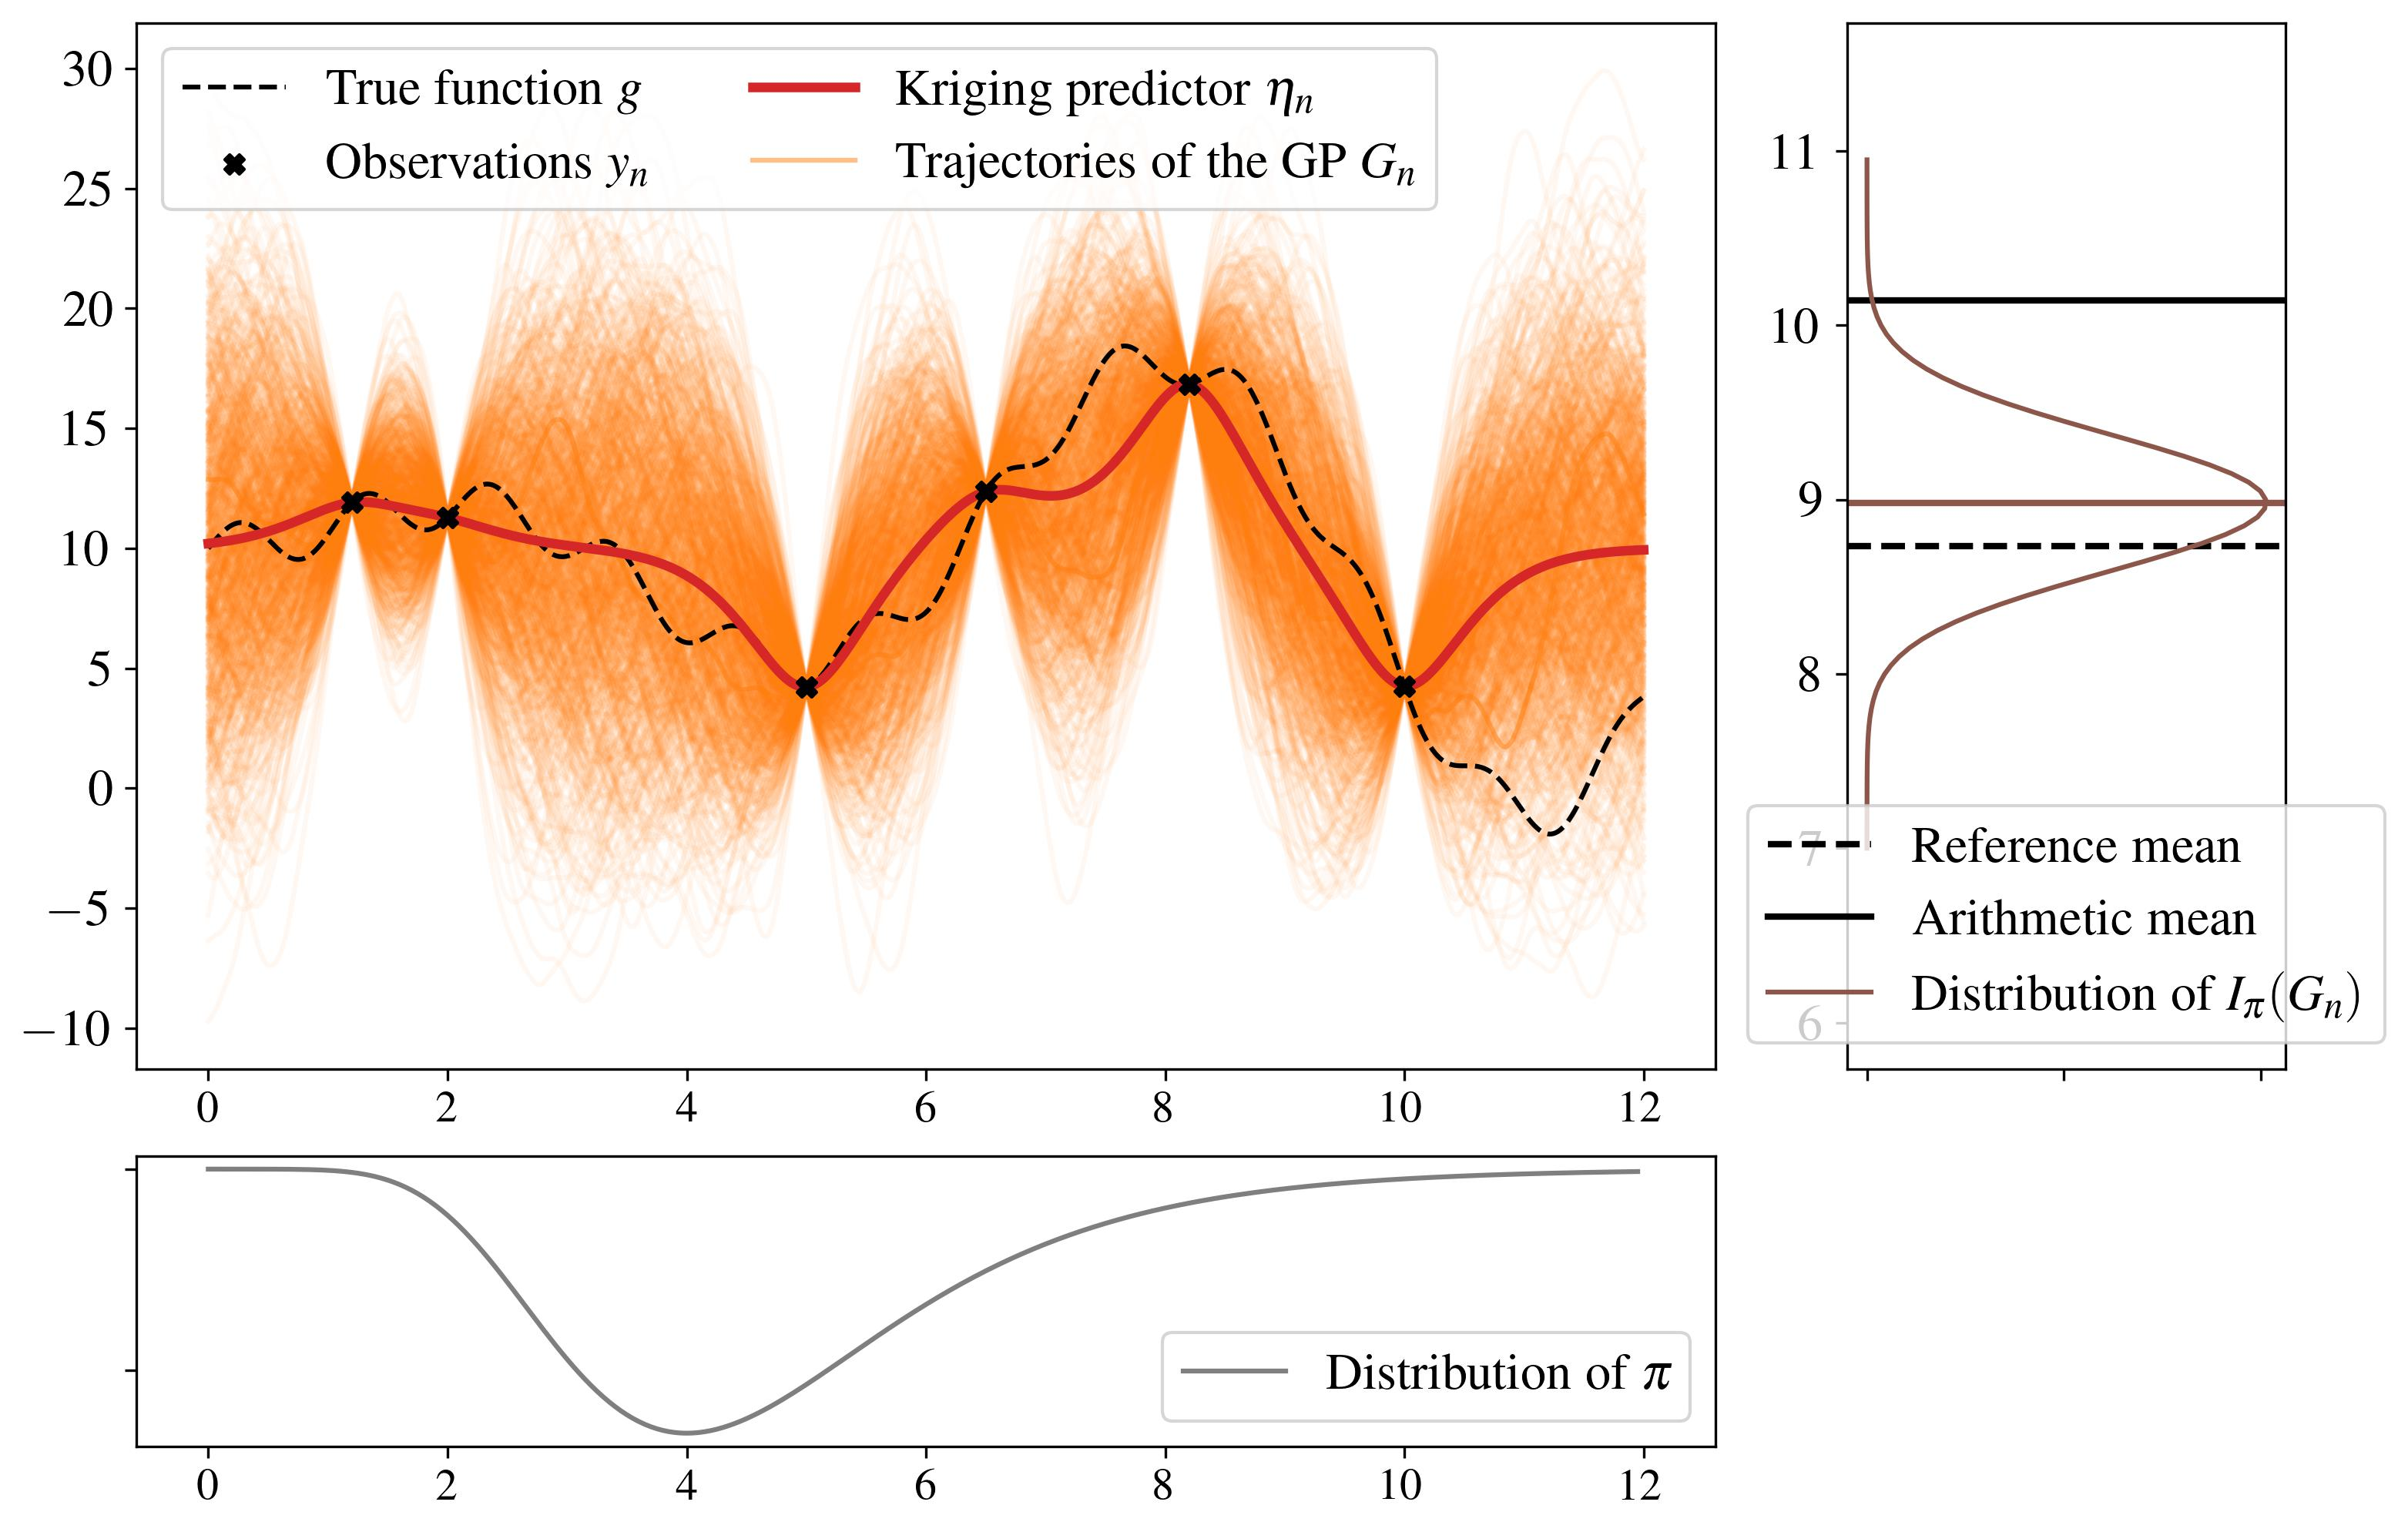
\includegraphics[width=0.7\textwidth]{part2/figures/DCE/numerical_experiments/posterior_distribution_centered.jpg}
    \caption{Bayesian quadrature on a one-dimensional case}
    \label{fig:bayesian_quad}
\end{center}
\end{figure}

\paragraph{Optimal weights computed by Bayesian quadrature}%---------------------%
Taking the random process $\xi_n$ as Gaussian conveniently implies that its posterior distribution $a_\mu(\xi_n)$ is also Gaussian. 
This comes from the linearity of the infinite sum of realizations of a Gaussian process. 
The posterior distribution is described in a closed form through its mean and variance by applying Fubini's theorem (see the supplementary materials from \cite{briol_oates_2019} for the proof regarding the variance): %\elias{Add the full proof for the variance in appendix?}:
\begin{equation}
     \bar{y}_n^{\mathrm{BQ}} := \E\left[I_{\mu}(\xi_n) | \by_n \right] 
     = \int_{\iD_\bX} \eta_n(\bx) \dd \mu(\bx)
     = \left[\int_{\iD_\bX} \bk_n\TT(\bx) \dd \mu(\bx) \right] \bK_n^{-1} \by_n
     = P_\mu(\bX_n) \bK_n^{-1} \by_n,       
\label{eq:mean_post}
\end{equation}

\begin{equation}
    \left(\sigma_n^{\mathrm{BQ}}\right)^2 := \var\left(I_{\mu}(\xi_n) \right) 
    = \iint_{\iD_{\bX^2}} k_n(\bx, \bx') \dd \mu(\bx) \dd \mu(\bx') 
    = \varepsilon_\mu - P_\mu(\bX_n) \bK_n^{-1} P_\mu(\bX_n)\TT.
\label{eq:var_post}
\end{equation}
\noindent
Where $P_\mu(\bX_n)$ is the row vector of potentials $\left[\int k_n(\bx, \bx^{(1)}) \dd \mu(\bx), \dots, \int k_n(\bx, \bx^{(n)}) \dd \mu(\bx)\right]$, and $\varepsilon_\mu$ is given in \eq{eq:target_energy}. 
As in the one-dimensional example presented in \fig{fig:bayesian_quad}, the expected value of $I_{\mu}(\xi_n)$ expressed in \eq{eq:mean_post} is a direct estimator of the quantity of interest \eq{eq:quadrature_rule}. 
The so-called ``Bayesian quadrature estimator'' appears to be a simple linear combination of the observations by taking the row vector of ``optimal weights'' as: 
\begin{equation}
    \wBQ := P_\mu(\bX_n) \bK_n^{-1}
    \label{eq:bq_weights}
\end{equation}
For any given sample, an optimal set of weights can be computed, leading to the mean of the posterior distribution. 
Remark here that this enhancement depends on the evaluation of the inverse variance-covariance matrix $\bK_n^{-1}$, which can present numerical difficulties, either when design points are too close, making the conditioning bad. 
Moreover, a prediction interval on the BQ estimator can be computed since the posterior distribution is Gaussian, with a variance expressed in closed-form in \eq{eq:var_post}. 
The expressions in \eq{eq:mean_post} and \eq{eq:var_post} were extended to Gaussian processes in the case of constant and linear trends in \cite{pronzato_zhigljavsky_2020}. 
In the following numerical experiments, the expression with a hypothesis of constant trend $\beta_n$ is used, which leads to:
\begin{equation}
     \E\left[I_{\mu}(\xi_n)\right] = \beta_n + P_\mu(\bX_n) \bK_n^{-1} \left(\by_n - \beta_n \mathbf{1}_n \right).
     \label{eq:mean_post_cst}
\end{equation}

\noindent Then, an a posteriori 95\% prediction interval around the mean Bayesian estimator is directly given by: 
\begin{equation}
   \Bar{y}_n^{\mathrm{BQ}} \in \left[\Bar{y}_n^{\mathrm{BQ}} - 2\sigma_n^{\mathrm{BQ}}, \Bar{y}_n^{\mathrm{BQ}} + 2\sigma_n^{\mathrm{BQ}} \right].
\end{equation}

\paragraph{Variance-based Bayesian quadrature rule}%----------------%
The link between the posterior variance and the squared MMD has been first made by \cite{husar_duvenaud_2012} in their Proposition 1: the expected variance in the Bayesian quadrature $\var\left(I_{\mu}(\xi_n)\right)$ is the MMD between the target distribution $\mu$ and $\zeta_n = \sum_{i=1}^n \wBQ^{(i)} \delta(\bx^{(i)})$. 
The proof is reproduced below (as well as in Proposition 6.1 from \cite{motonobu_2018}): %\elias{check the condition to the Huszar's demonstration}
\begin{subequations}
\begin{align}
    \var\left(I_{\mu}(\xi_n)\right) &= \E\left[ \left(I_{\mu}(\xi_n) - I_{\zeta_n}(\xi_n)\right)^2\right]\\
    &= \E\left[ \left( \left\langle \xi_n, P_{\mu} \right\rangle_{\iH(k)} - \left\langle \xi_n, P_{\zeta_n}\right\rangle_{\iH(k)} \right)^2\right]\\
    &= \E\left[ \left\langle \xi_n, P_{\mu} - P_{\zeta_n} \right\rangle_{\iH(k)}^2\right]\\
    %&= \E\left[ \lVert \xi_n \lVert^2 + \lVert P_{\mu}(\bx) - P_{\zeta_n}(\bx) \lVert^2 - 2 \left\langle \xi_n, P_{\mu}(\bx) - P_{\zeta_n}(\bx) \right\rangle_{\iH(k)}\right]\\
    &= \lVert P_{\mu} - P_{\zeta_n} \lVert^2_{\iH(k)}\\ 
    &= \MMD_k(\mu, \zeta_n)^2.
\end{align}
\end{subequations}
Note that the transition from equation (27c) to (27d) relies on the property stating that if $\xi$ is a standard Gaussian process then $\forall g \in \iH(k) : \left\langle \xi, g \right\rangle_{\iH(k)} \sim \iN(0, \lVert g \lVert^2_{\iH(k)}$). 
The method that sequentially builds a quadrature rule by minimizing this variance is called by the authors ``Sequential Bayesian Quadrature'' (SBQ). 
According to the previous proof, this criterion can be seen as an optimally-weighted version of the kernel herding criterion, as stated in the title of the paper from \cite{husar_duvenaud_2012}. 
Later, \cite{briol_2015} proved the weak convergence of $I_{\mu}(\xi_n)$ towards the target integral. 
Closer to wind turbines applications, \cite{huchet_2019} and \cite{huchet_mattrand_2019} introduced the ``Adaptive Kriging Damage Assessment'' method: a Kriging-based method for mean damage estimation that is very close to SBQ. 
However, This type of method inherits the limits from both KH and BQ since it searches for optimal design points among a candidate set and computes an inverse variance-covariance matrix. 
These numerical operations both scale hardly in high dimension. 

\medskip
\begin{remark}
Every quadrature method introduced in this section has been built without any observation of the possibly costly function $g$. 
Therefore, they cannot be categorized as active learning approaches. 
Contrarily, \cite{motonobu_2019} presents a set of methods for BQ with transformations (i.e., adding a positivity constraint on the function $g$), which are truly active learning methods. 
\end{remark}

%In the end, active methods are not widely used for numerical integration \citep{wei_2020,goncalves_batchvarov_2020}, and from a general point of view, one can wonder in which situation the active learning framework presents a actual added value. 

%Apart from some very specific problems (e.g., contour finding of a limit-state function in reliability analysis \citep{echard_2011}. 

%\begin{remark}
%As much as the previous criteria will reduce the posterior variance, the estimation error may present a bias.
%\end{remark}

%============================================================%
%============================================================%
\section{Numerical experiments}\label{sec4}
%============================================================%
%============================================================%

This section presents numerical results computed on two different analytical toy-cases, respectively in dimension 2 (toy-case \#1) and dimension 10 (toy-case \#2), with easy-to-evaluate functions $g(\cdot)$ and associated input distributions $\mu$. 
Therefore, reference values can easily be computed with great precision. 
For each toy-case a large reference Monte Carlo sample ($N_{\mathrm{ref}} = 10^8)$ is taken. 
This first benchmark compares the mean estimation of toy-cases given by quasi-Monte Carlo Sobol' sequences (abbreviation by QMC in the next figures), and kernel herdings with the three kernels defined in Table \ref{tab:kernels}. 
Notice that the quasi-Monte Carlo designs are first generated on the unit cube, then transformed using the generalized Nataf transformation to follow the target distribution \citep{lebrun_2009}. 
Additionally, the performances of kernel herding for both uniform and optimally-weighted \eq{eq:mean_post_cst} estimators are compared. 

The kernel-based sampling and BQ methods were implemented in a new open-source Python package named \texttt{otkerneldesign\footnote{\href{https://efekhari27.github.io/otkerneldesign/master/index.html}{https://efekhari27.github.io/otkerneldesign/master/index.html}}}. 
This development mostly relies on OpenTURNS\footnote{\href{https://openturns.github.io/www/}{https://openturns.github.io/www/}}, an ``Open source initiative for the Treatment of Uncertainties, Risks'N Statistics'', see \cite{baudin_dutfoy_2017}. 
The following numerical experiments are available in the Git repository named \texttt{ctbenchmark}\footnote{\href{https://github.com/efekhari27/ctbenchmark}{https://github.com/efekhari27/ctbenchmark}}. 


%------------------------------------------------------------%
\subsection{Illustration through analytical toy-cases}
%------------------------------------------------------------%
%\emph{Toy-case 1. } $g_1(\bx)= x_1 + x_2$, with a complex Gaussian mixture as input random variable (which density is represented by the iso-probability contours in \fig{fig:KH_mixture}). 
%\emph{Toy-case 2.} $g_2(\bx) = \prod_{i=1}^10 \frac{|4 x_i - 2| + a_i}{1 + a_i}, a_i = 2$, also referred to as ``G-Sobol'' function, with a normal input random variable $\iN(\mathbf{0.5},\mathbf{I}_5)$. 
The toy-cases were chosen to cover a large panel of complex probabilistic integration problems, completing the ones from \cite{fekhari_renew_2021}.
To assess the complexity of numerical integration problems, \cite{owen_2003} introduced the concept of the ``effective dimension'' of an integrand function (number of the variables that actually impact the integral). 
The author showed that functions built on sums yield a low effective dimension (unlike functions built on products). 
In the same vein, \cite{kucherenko_feil_2011} build three classes of integrand sorted by difficulty depending on their effective dimension: \begin{itemize}
    \item \emph{class A}: problem with a few dominant variables.
    \item \emph{class B}: problem without unimportant variables, and important low-order interaction terms.
    \item \emph{class C}: problems without unimportant variables, and important high-order interaction terms. 
\end{itemize}
The 10-dimensional ``GSobol function'' (toy-case \#2) with a set of coefficient $\{a_i=2\}_{i=1}^{10}$ has an effective dimension equal to 10 and belongs to the hardest class C from \cite{kucherenko_feil_2011}. 
In the case of the two-dimensional Gaussian mixture problem, the complexity is carried by the mixture of Gaussian distributions with highly nonlinear dependencies.
Probabilistic integration results are presented in \fig{fig:toy-case1} (toy-case \#1) and \fig{fig:toy-case2} (toy-case \#2). 
Kernel herding samples with kernels defined in Table \ref{tab:kernels} (squared exponential in green, Matérn in orange, and energy-distance in red), are compared with a quasi-Monte Carlo sample (Sobol' sequences in grey). 
Convergences of the arithmetic means are plotted on the left and MMDs on the right. 
The respective BQ estimators of the means are plotted in dashed lines. 

\begin{table*}[h]
    \centering
    \caption{Analytical toy-cases}
    \begin{tabular}{llll}
     \hline
        \textbf{Toy-case \#1} & $dim = 2$ & $g_1(\bx)= x_1 + x_2$ & Gaussian mixture from \fig{fig:KH_mixture} \\
        \textbf{Toy-case \#2} & $dim = 10$ & $g_2(\bx) = \prod_{i=1}^{10} \frac{|4 x_i - 2| + a_i}{1 + a_i}, \{a_i=2\}_{i=1}^{10}$ & Gaussian $\iN(\mathbf{0.5},\mathbf{I}_{10})$\\
    \end{tabular}
    \label{tab:toycases}
\end{table*}

\medskip
\begin{remark}
Different kernels are used in these numerical experiments. 
First, the generation kernel, used by the kernel herding algorithm to generate designs (with the heuristic tuning defined in Section \ref{sec:khsubsec}). 
Second, the BQ kernel allows computation of the optimal weights (arbitrarily set up as a Matérn $5/2$ with the heuristic tuning). 
Third, the evaluation kernel, which must be common to allow a fair comparison of the computed MMD results (same as the BQ kernel).
\end{remark}
\medskip

\noindent\emph{About toy-case \#1.} KH consistently converges faster than quasi-Monte Carlo in this case, especially for small sizes in terms of MMD. 
BQ weights tend to reduce the fluctuations in the mean convergence, which ensures better performance for any size. 
Overall, applying the weights enhances to convergence rate.

\smallskip
\noindent\emph{About toy-case \#2.} Although quasi-Monte Carlo is known to suffer the ``curse of dimensionality'', KH does not outperform it drastically in this example. 
In fact, KH with uniform weights performs worse than quasi-Monte Carlo while optimally-weighted KH does slightly better. 
Moreover, the results confirm that $\MMD_{\mathrm{BQ}}< \MMD_{\mathrm{unif}}$ for all our experiments. 
The application of optimal-weights to the quasi-Monte Carlo sample slightly improves the estimation on this case. 
Note that the prediction interval around the BQ estimator is not plotted for the sake of readability. 
\smallskip

In these two toy-cases, the MMD is shown to quantify numerical integration convergence well, which illustrates the validity of the inequality given in \eq{eq:quad_error}, similar to the Koksma-Hlawka inequality, recalled in \eq{eq:KH_inequality}.

%\begin{figure}[!h]
%\begin{center}
%    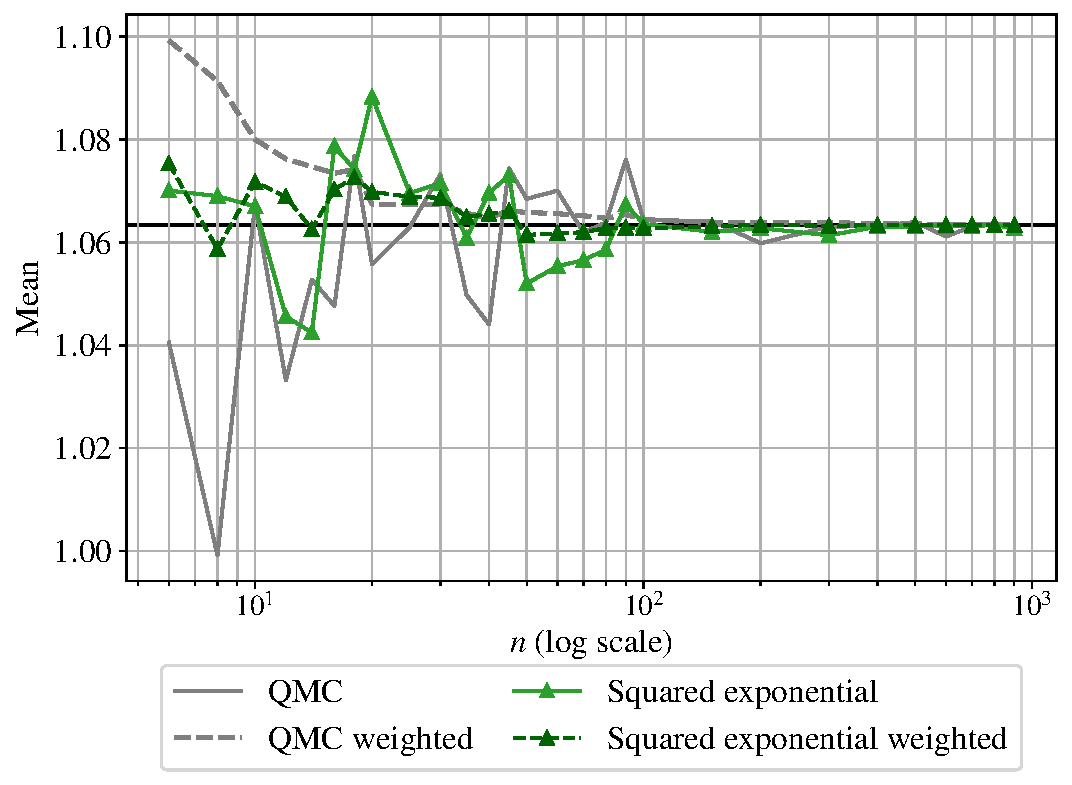
\includegraphics[width=0.48\textwidth]{part2/figures/DCE/analytical_bench/Gaussian Mixture_convergence_SE.pdf}
%    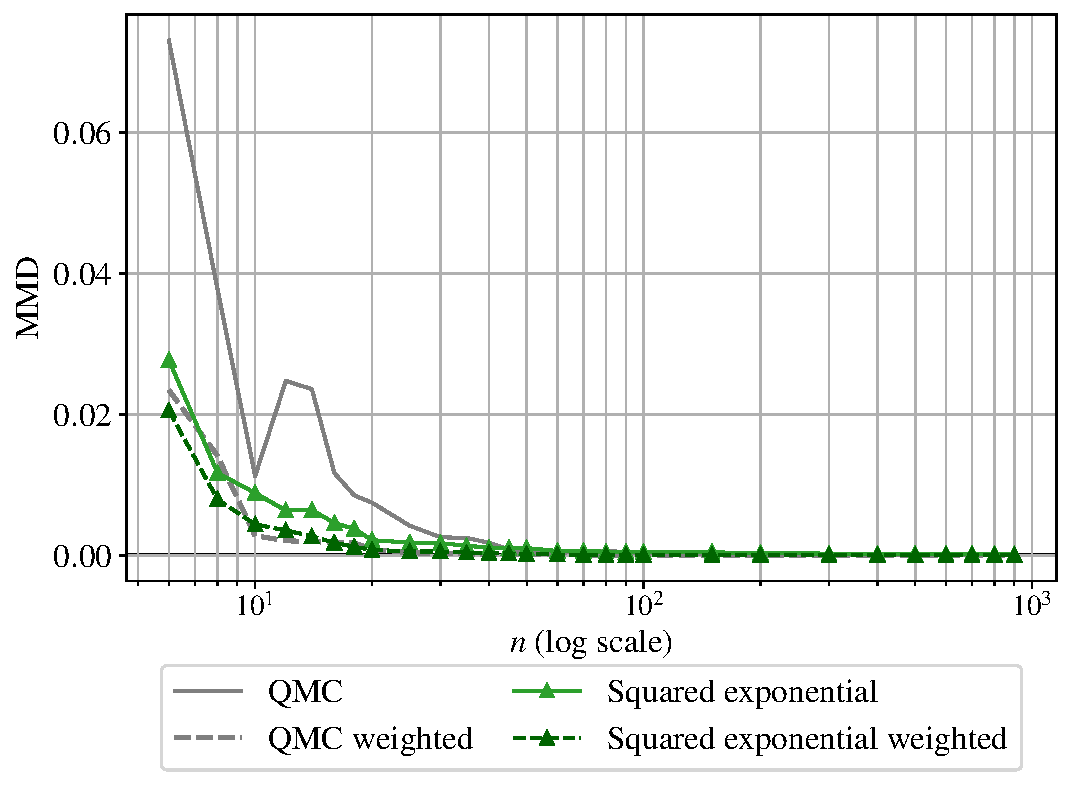
\includegraphics[width=0.48\textwidth]{part2/figures/DCE/analytical_bench/Gaussian Mixture_convergence_MMD_SE.pdf}\\
%    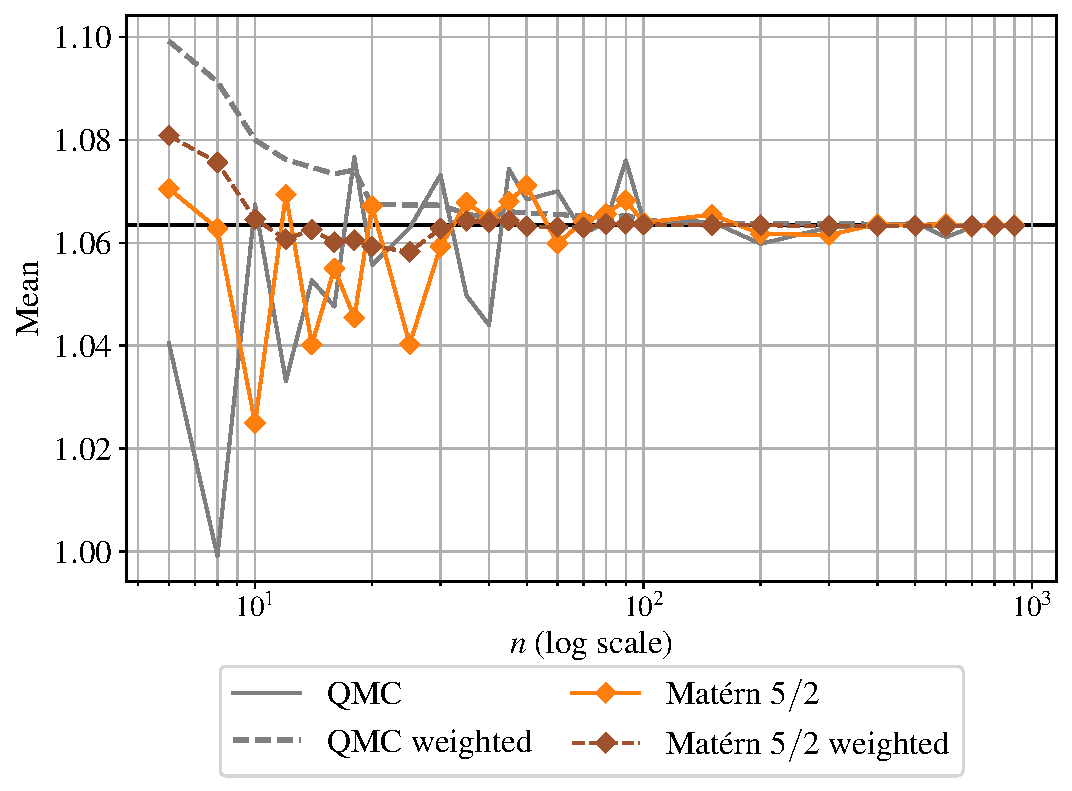
\includegraphics[width=0.48\textwidth]{part2/figures/DCE/analytical_bench/Gaussian Mixture_convergence_Matern.pdf}
%    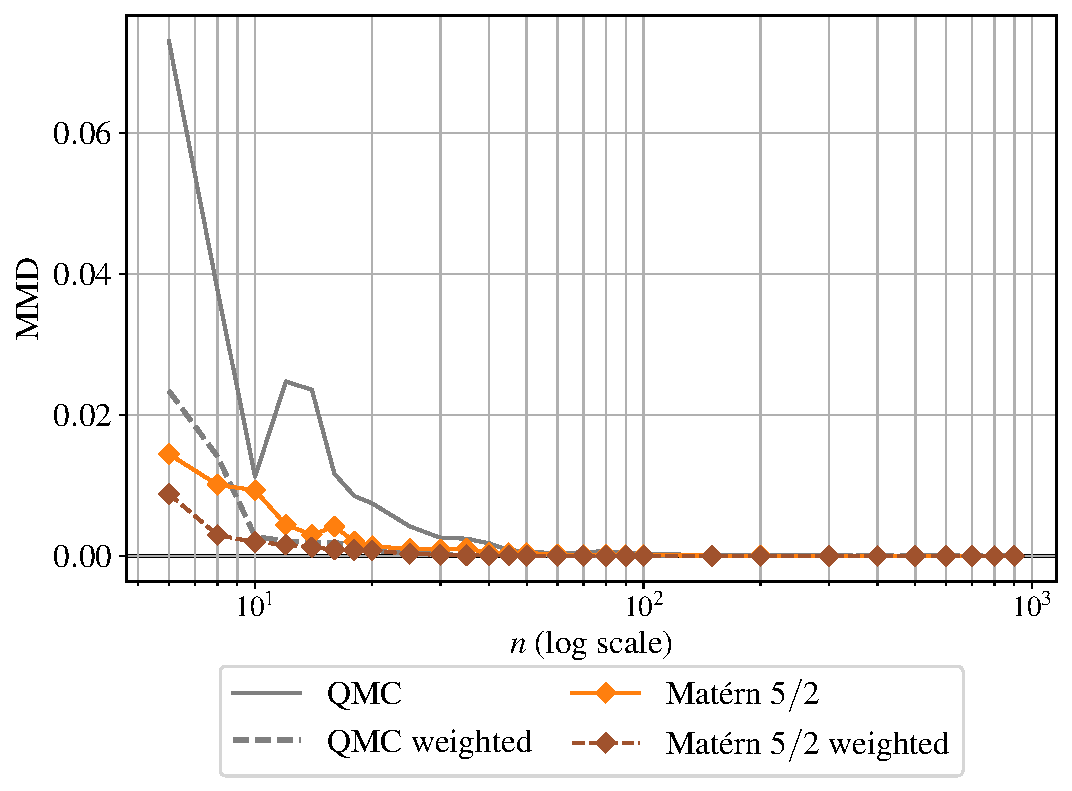
\includegraphics[width=0.48\textwidth]{part2/figures/DCE/analytical_bench/Gaussian Mixture_convergence_MMD_Matern.pdf}\\
%    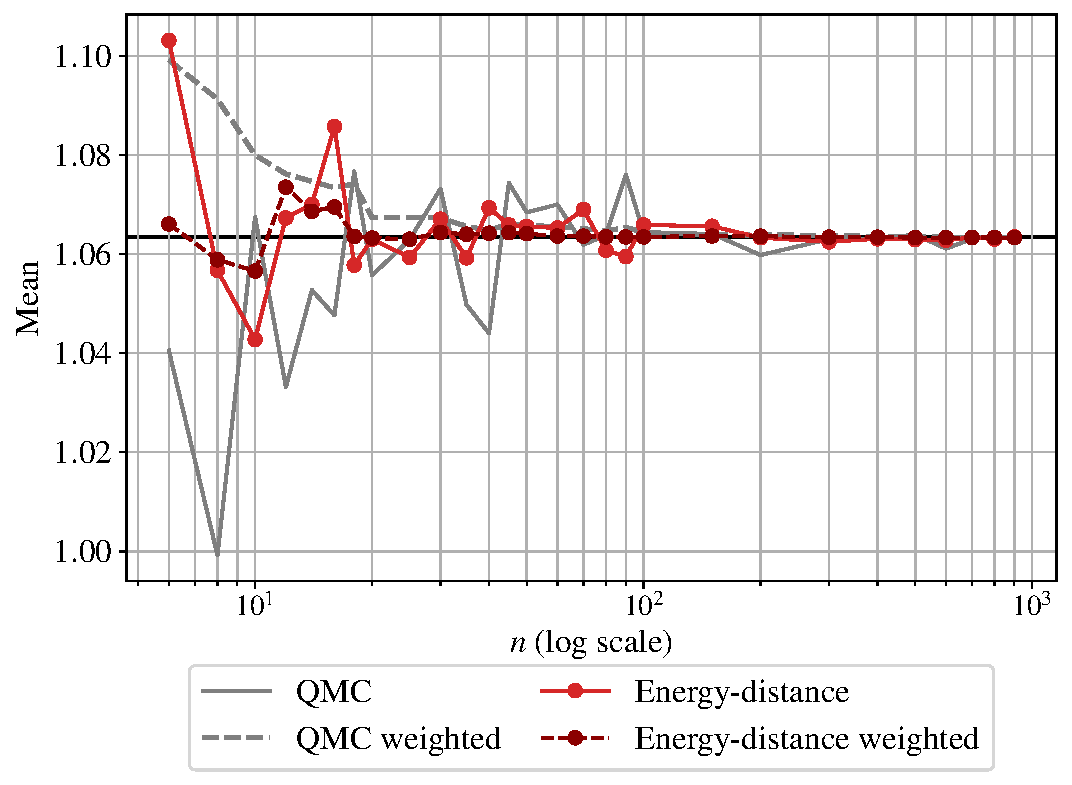
\includegraphics[width=0.48\textwidth]{part2/figures/DCE/analytical_bench/Gaussian Mixture_convergence_ED.pdf}
%    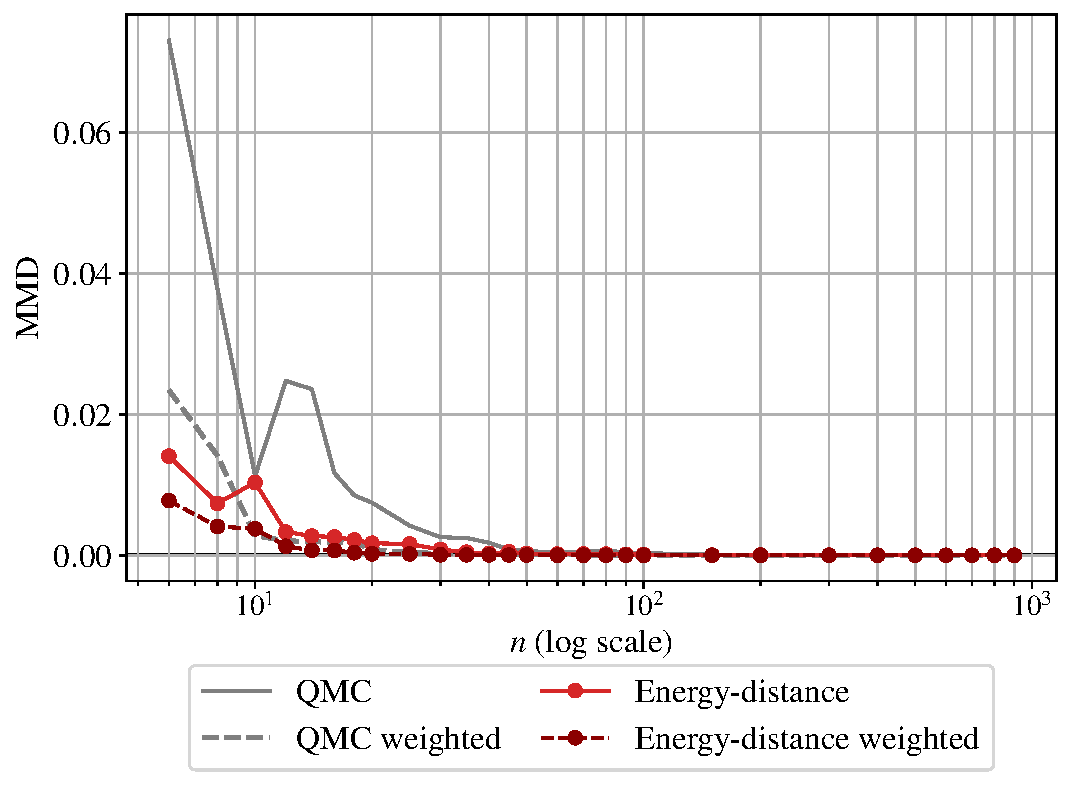
\includegraphics[width=0.48\textwidth]{part2/figures/DCE/analytical_bench/Gaussian Mixture_convergence_MMD_ED.pdf}\\
%\end{center}
%\caption{Analytical benchmark results on the toy-case \#1} \label{fig:toy-case1}
%\end{figure}
%
%\begin{figure}[!h]
%\begin{center}
%    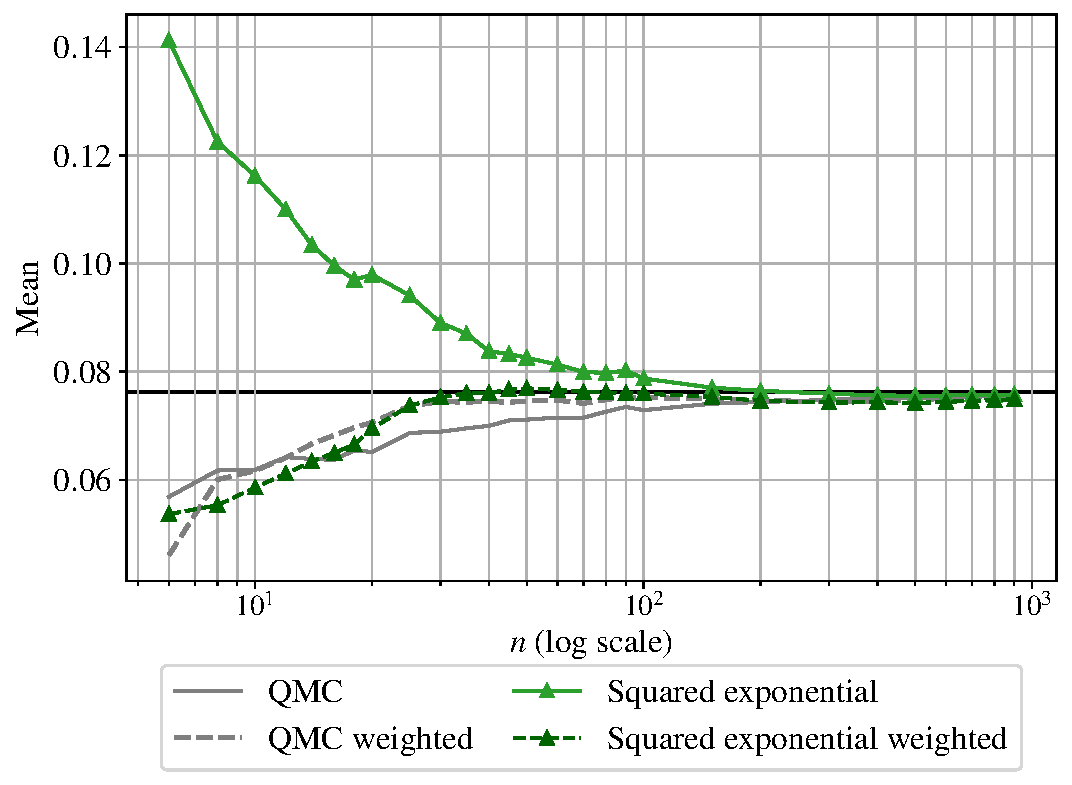
\includegraphics[width=0.48\textwidth]{part2/figures/DCE/analytical_bench/GSobol 10D (normal input)_convergence_SE.pdf}
%    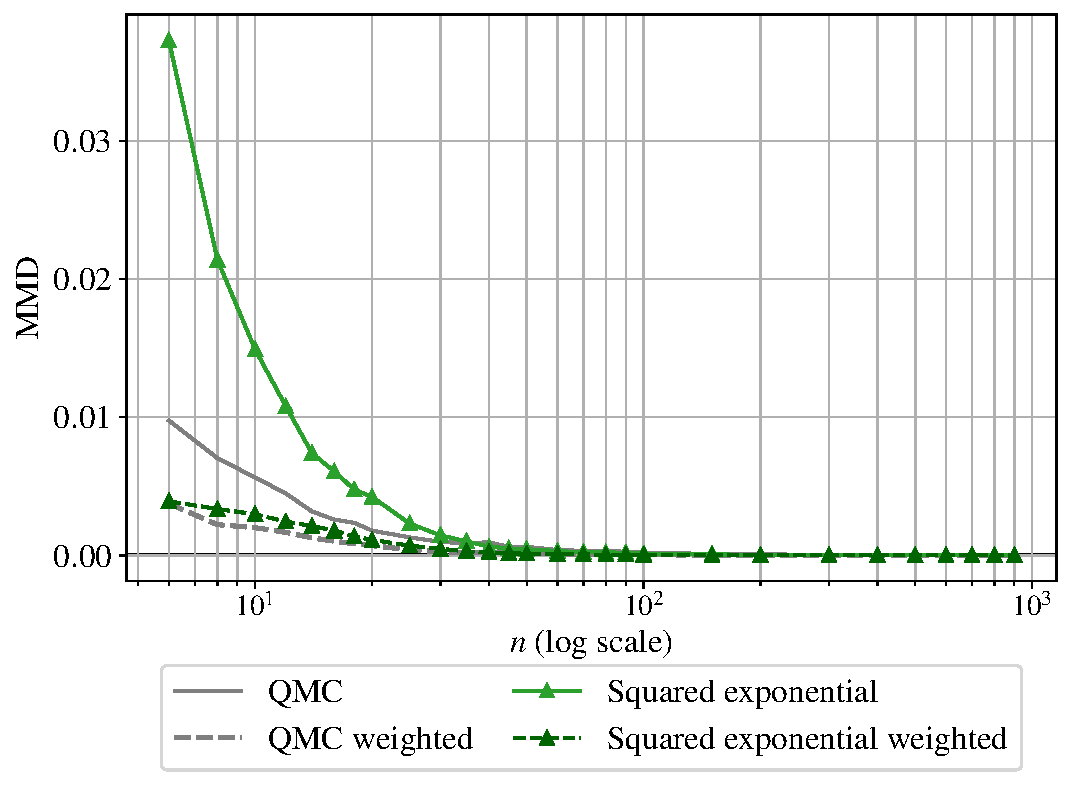
\includegraphics[width=0.48\textwidth]{part2/figures/DCE/analytical_bench/GSobol 10D (normal input)_convergence_MMD_SE.pdf}\\
%    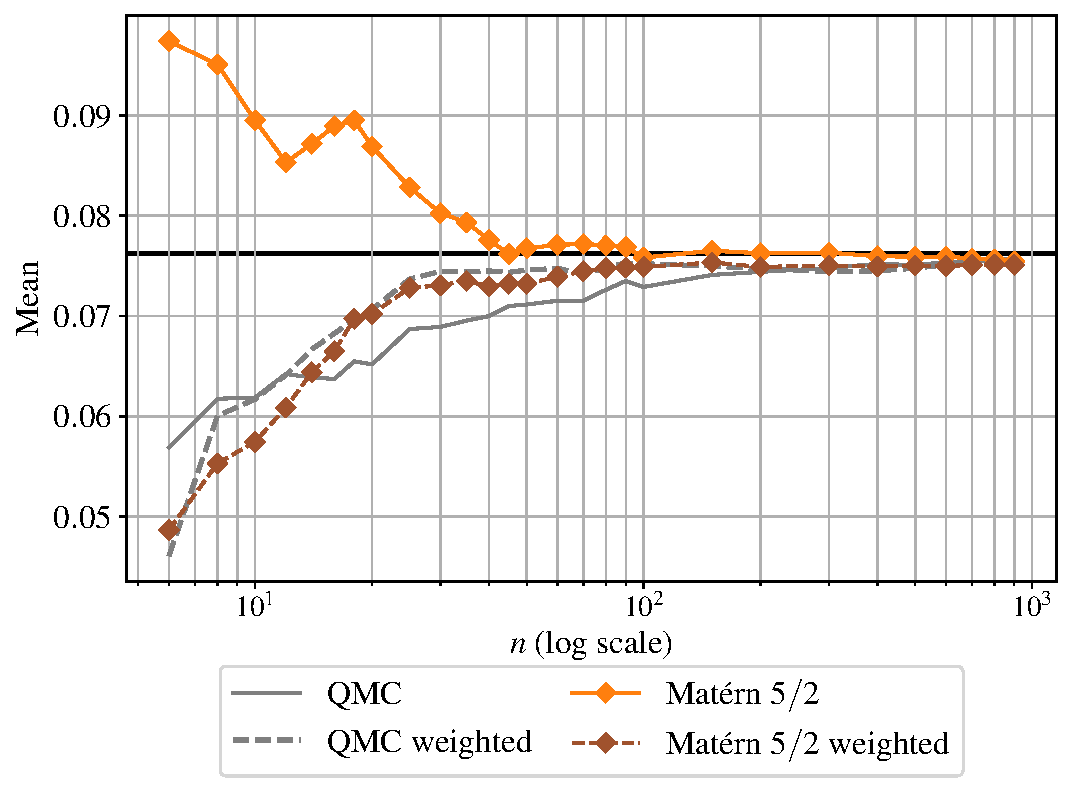
\includegraphics[width=0.48\textwidth]{part2/figures/DCE/analytical_bench/GSobol 10D (normal input)_convergence_Matern.pdf}
%    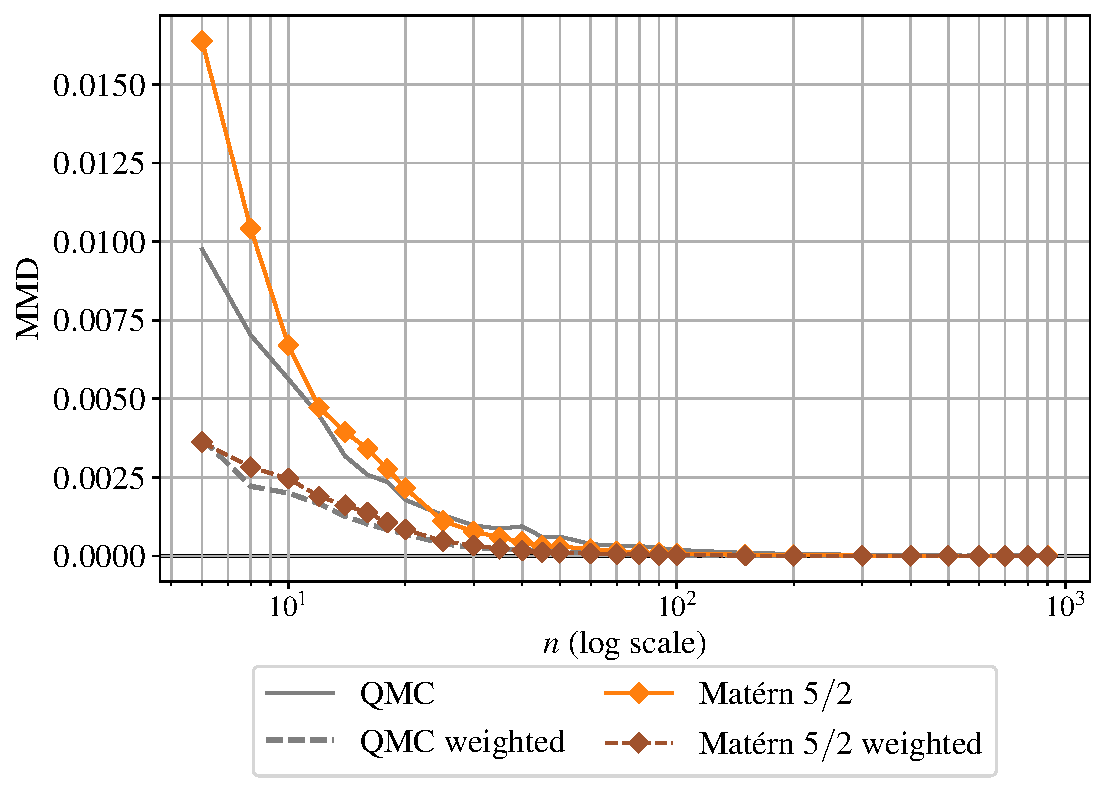
\includegraphics[width=0.48\textwidth]{part2/figures/DCE/analytical_bench/GSobol 10D (normal input)_convergence_MMD_Matern.pdf}\\
%    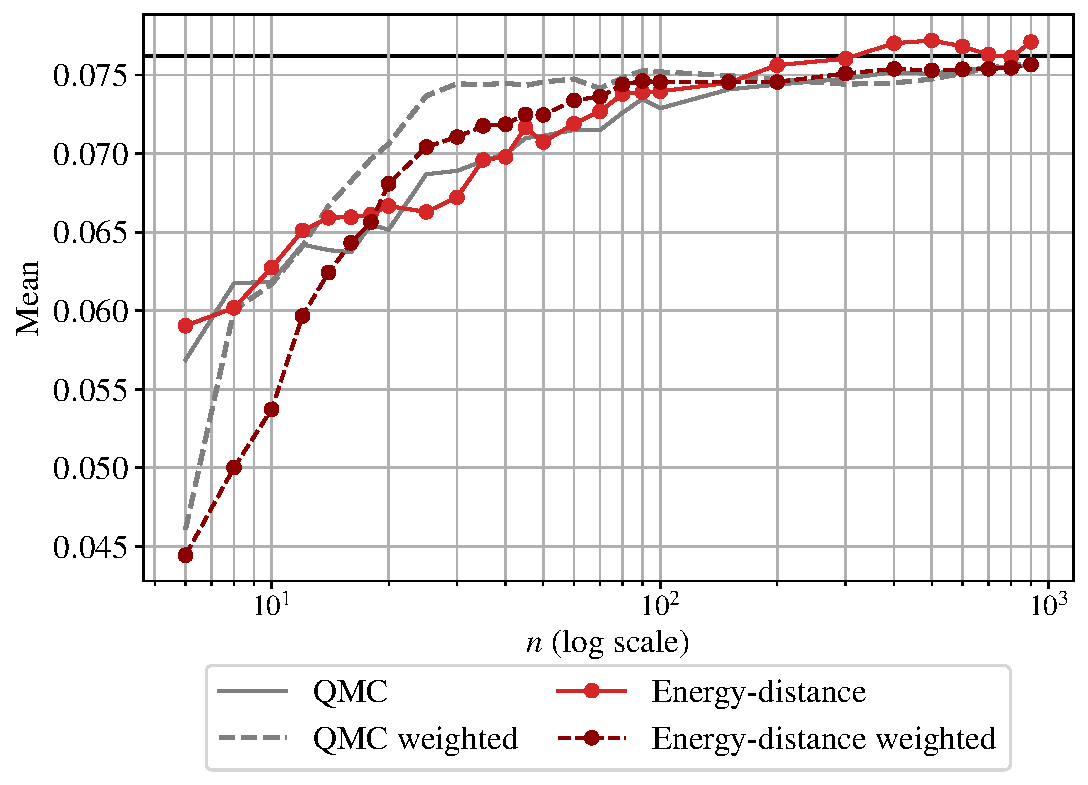
\includegraphics[width=0.48\textwidth]{part2/figures/DCE/analytical_bench/GSobol 10D (normal input)_convergence_ED.pdf}
%    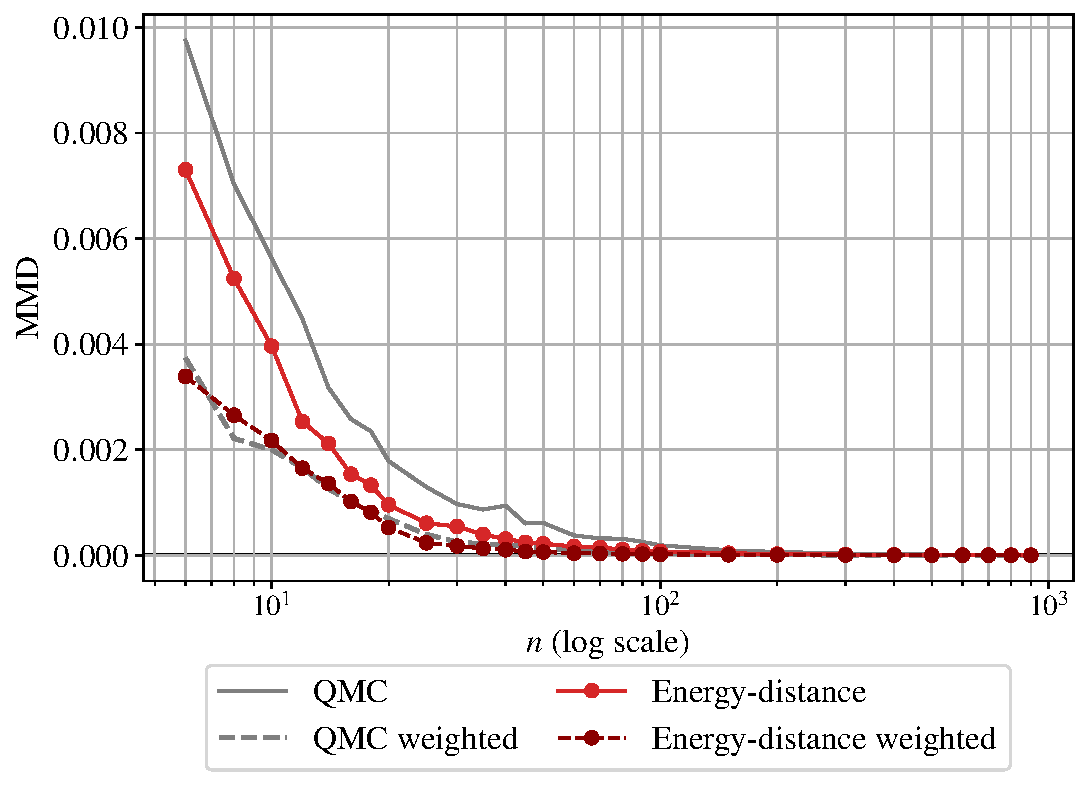
\includegraphics[width=0.48\textwidth]{part2/figures/DCE/analytical_bench/GSobol 10D (normal input)_convergence_MMD_ED.pdf}\\
%\end{center}
%\caption{Analytical benchmark results on the toy-case \#2} \label{fig:toy-case2}
%\end{figure}

%----------------------------------------------------------------------%
\subsection{Application to the Teesside wind turbine fatigue estimation}
%----------------------------------------------------------------------%

Before analyzing the performance of the KH on the industrial application, let us notice that the copulogram \fig{fig:pairplot_kh_teesside} seems to be in line with the global sensitivity analysis presented in \cite{murcia_dimitrov_2018} and \cite{li_zhan_2020}. 
In particular, the fact that the scatter plot of mean wind speed vs. turbulence wind speed is the main factor explaining the variance of the output $Y=g(\bX)$. 
Judging from these references, the numerical model does not seem to have high effective dimension, however, the input dependence structure is challenging and the damage assessment induces strong nonlinearities (see \eq{eq:wohler}). 

Crude Monte Carlo and kernel herding both subsample directly from a large dataset (previously referred to as candidate set). 
Unlike them, quasi-Monte Carlo generates a uniform sample in the unit hypercube, which can then be transformed according to a target distribution. 
In our case, this distribution is only known empirically via the candidate set. 
Since its dependence structure is complex (see \fig{fig:envi_pairplot}), a parametric model might fit the distribution poorly (and therefore lead to a poor quasi-Monte Carlo estimation of the quantity). 
Then, a nonparametric fit using the empirical Bernstein copula (introduced in Section \ref{sec:ebc}) coupled with a kernel density estimation on each marginal is applied to the candidate set (with the EBC parameter $m=100 > m_{MISE}$ to avoid bias). 
Subsequently, quasi-Monte Carlo sampling is applied to this nonparametric model. 
These two approaches are summarized in \fig{fig:sampling_diagram}, showing a practical advantage to the subsampling methods.

\begin{figure}[!h]
    \centering
    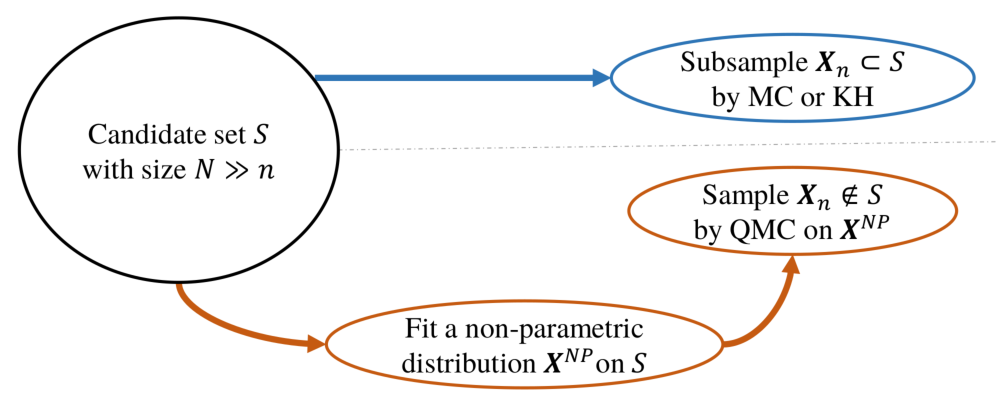
\includegraphics[width=0.6\textwidth]{part2/figures/DCE/diagram_samplings.pdf}
    \caption{Sampling techniques used for the industrial use case}
    \label{fig:sampling_diagram}
\end{figure}

The results presented are compared in the following to a reference Monte Carlo sample with a confidence interval computed by bootstrap (see \fig{fig:convergence_teesside}). 
The performance of the KH is good: it quickly converges towards the confidence interval of the Monte Carlo obtained with the reference sample. 
In addition, the Bayesian quadrature estimator also offers a posteriori prediction interval, which can reassure the user. 
The BQ prediction intervals are smaller that the ones obtained by bootstrap on the reference Monte Carlo sample. 
To provide more representative results, note that a set of scale parameters is computed with a kriging procedure to define the kernel used to compute BQ intervals. 
Since other methods do not generate independent samples, bootstrapping them is not legitimate. 
Contrarily to the other kernel, we observe that the energy-distance kernel presents a small bias with the MC reference for most of the azimuth angles computed in this experiment. 
Finally, combining nonparametric fitting with quasi-Monte Carlo sampling also delivers good results as long as the fitting step does not introduce a bias. 


\begin{figure}[!h]
\begin{center}
    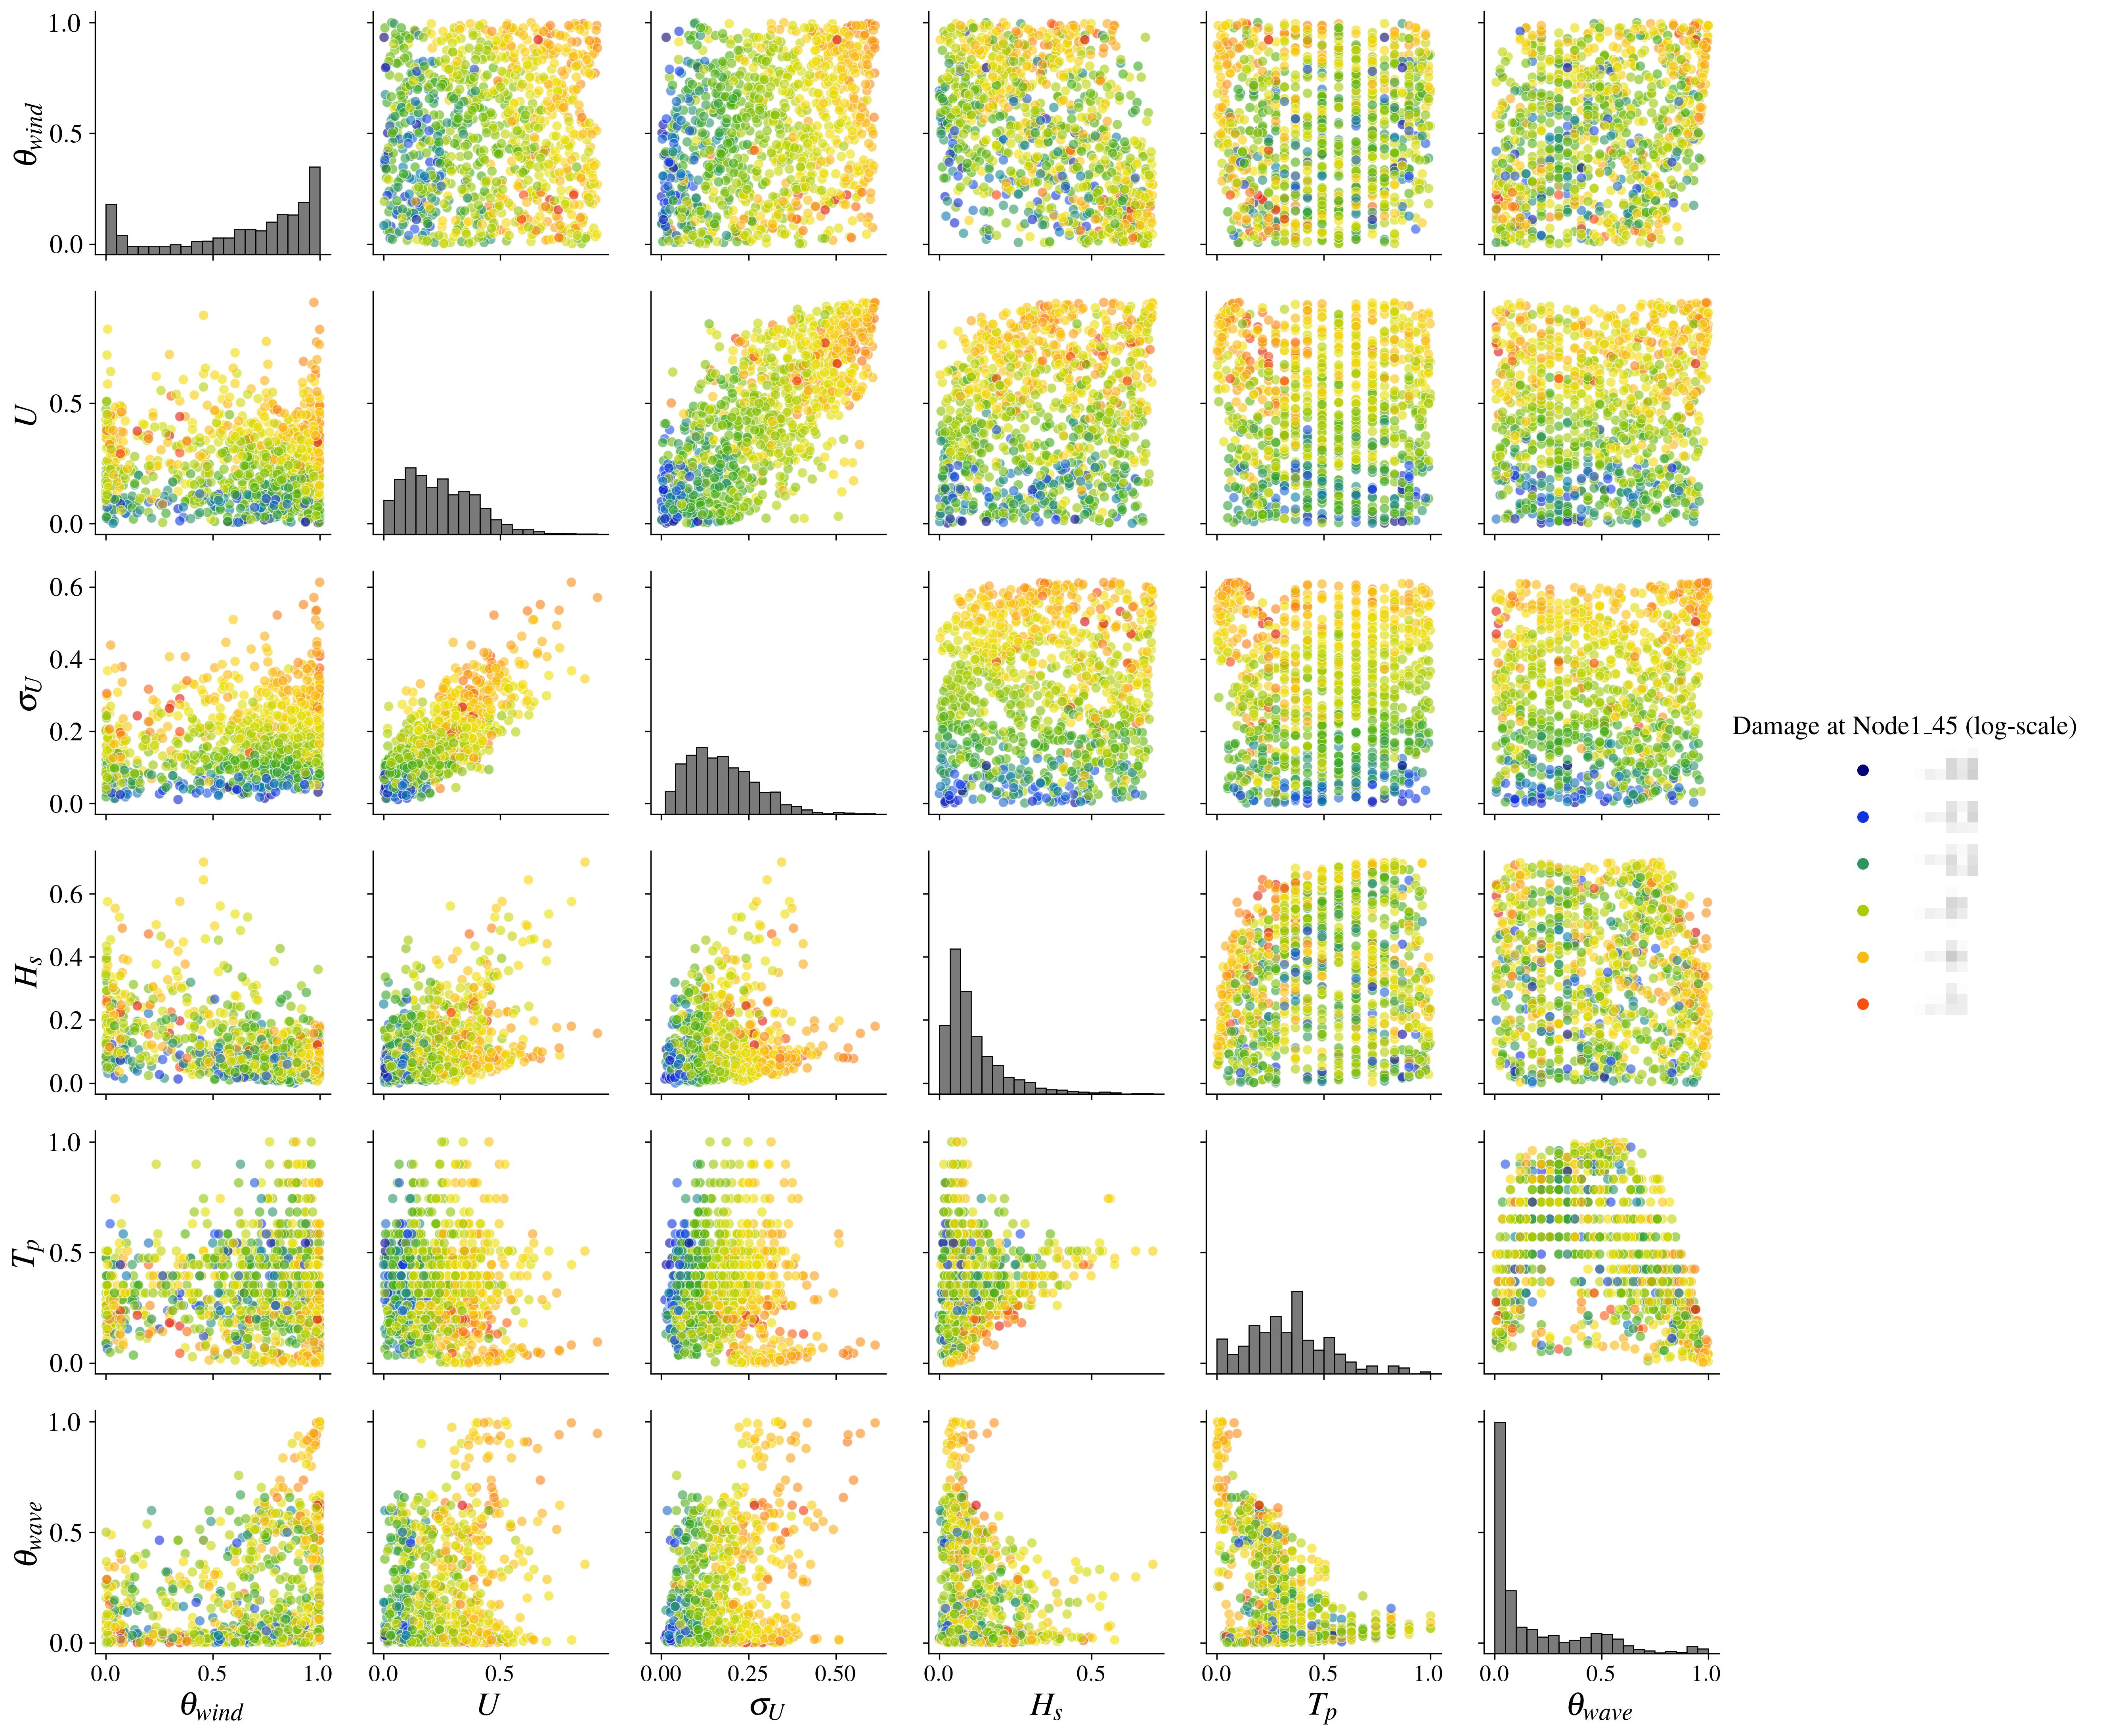
\includegraphics[width=\textwidth]{part2/figures/DCE/teesside/kh_output_pairplot.jpg}
\end{center}
\caption{Copulogram of the kernel herding design of experiments with corresponding outputs in color (log-scale) on the Teesside case ($n = 10^3$). 
The highest values are in red while the lowest values are in blue. 
Marginals are represented by histograms (diagonal), the dependence structure with scatter plots in the ranked space (upper triangle). 
Scatter plots on the bottom triangle are set in the physical space.} \label{fig:pairplot_kh_teesside}
\end{figure}

\begin{figure}[!h]
\begin{center}
    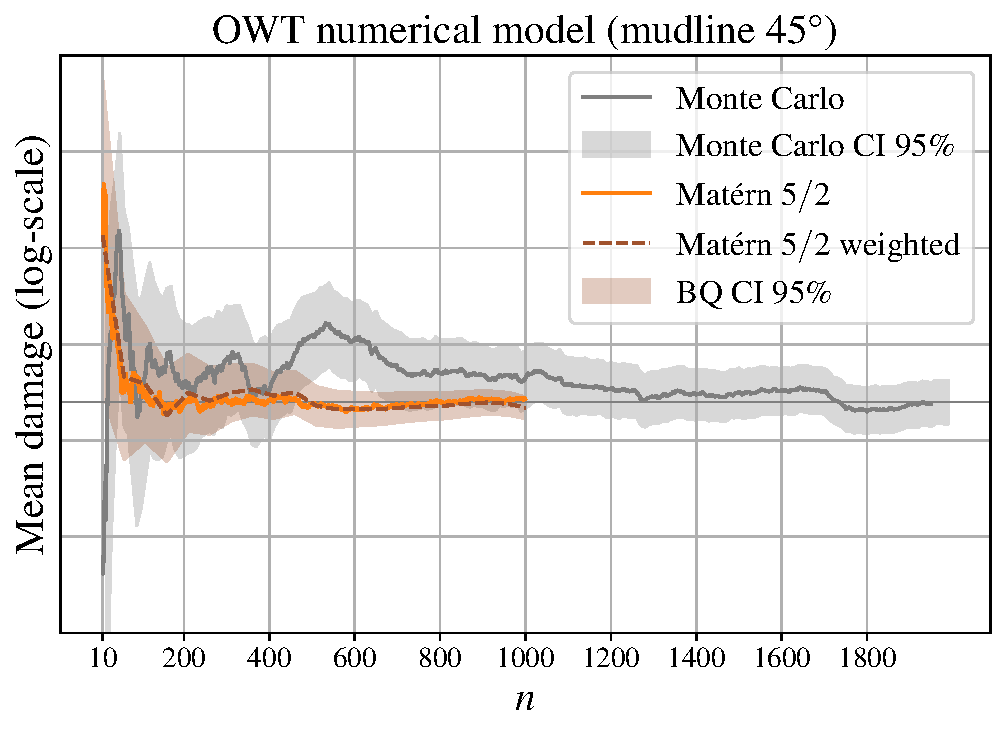
\includegraphics[width=0.49\textwidth]{part2/figures/DCE/teesside/log_convergence_MaternNode1_45.pdf}
    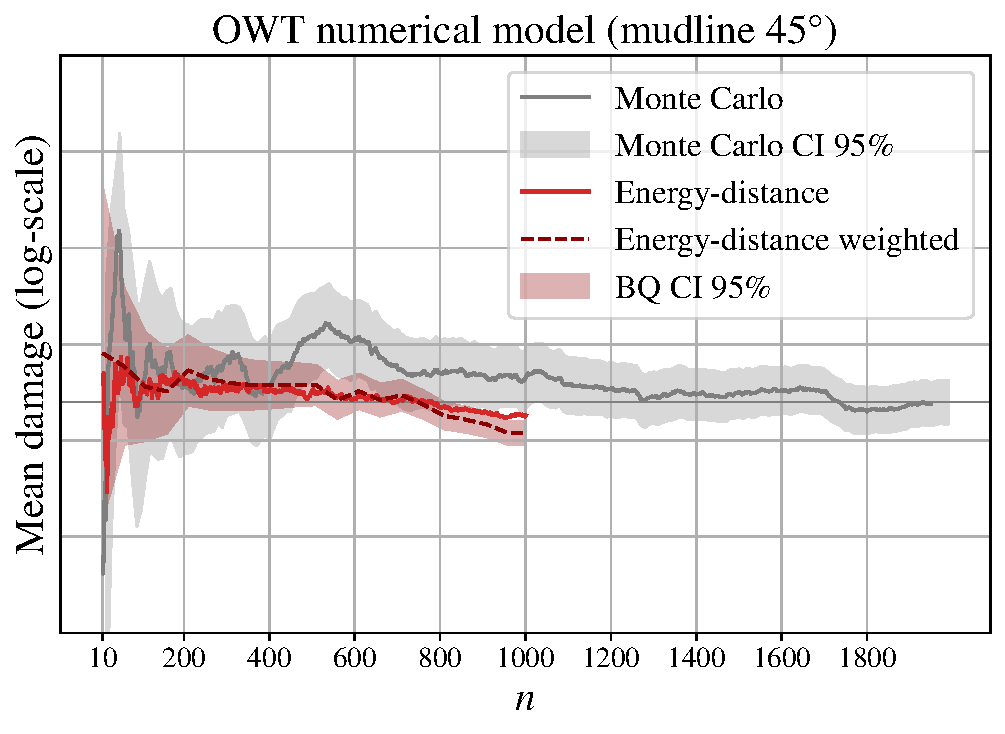
\includegraphics[width=0.49\textwidth]{part2/figures/DCE/teesside/log_convergence_EnergyNode1_45.pdf}
    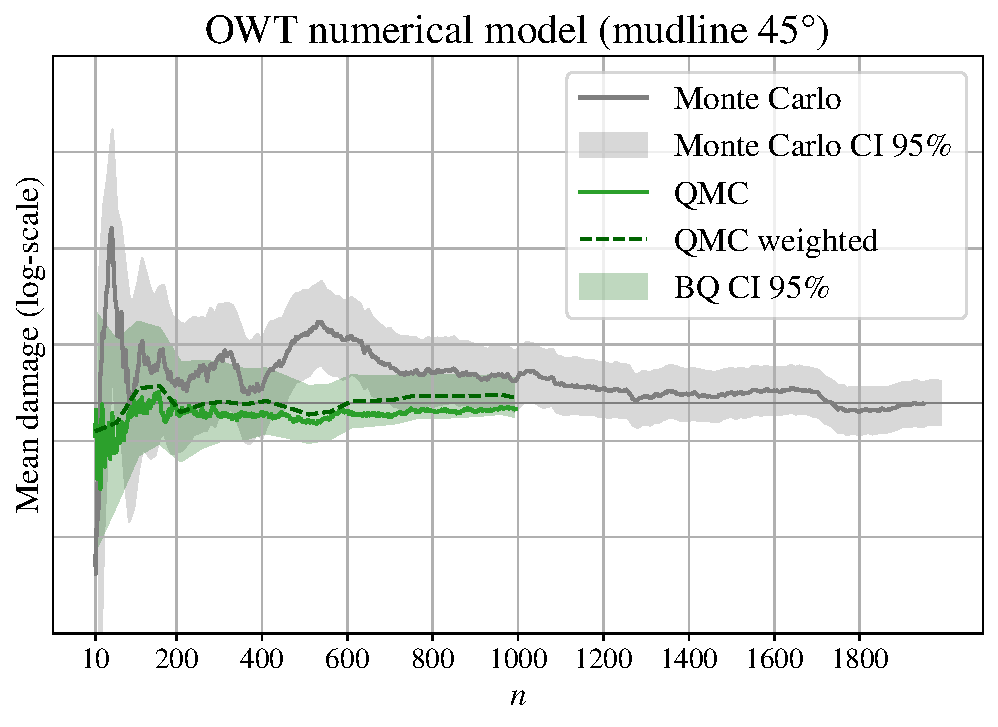
\includegraphics[width=0.49\textwidth]{part2/figures/DCE/teesside/log_convergence_QMCNode1_45.pdf}
\end{center}
\caption{Mean estimation convergence (at the mudline, azimuth $\theta=45~\mathrm{deg.}$) on the Teesside case} \label{fig:convergence_teesside}
\end{figure}


%============================================================%
%============================================================%
\section{Conclusion}\label{sec5}
%============================================================%
%============================================================%

Wind energy assets are subject to highly uncertain environmental conditions. 
Uncertainty propagation through numerical models is performed to ensure their structural integrity (and energy production). 
For this case, the method recommended by the standards (regular grid sampling) is intractable. 
This can lead, in practice, to poor uncertainty propagation under the constraint of a simulation budget. 
This industrial use case induces two practical constraints. 
First, active learning methods are hard to set up on such a numerical model, and they restrict the use of high-performance computers. 
Second, the input distribution of the environmental conditions presents a complex dependence structure, hard to model with parametric approaches. 

In this paper, the association of kernel herding sampling with Bayesian quadrature for central tendency has been both explored theoretically and numerically. 
This method fits with the practical constraints induced by the industrial use case. 
Kernel herding sampling subsamples the relevant points directly from a given dataset (here from the measured environmental data). 
Moreover, the method is fully compatible with intensive high-performance computer use. This work provides an MMD-based upper bound on numerical integration absolute error. 
Kernel herding and Bayesian quadrature both aim at finding the quadrature rule minimizing the MMD, and therefore the absolute integration error. 
The numerical experiments confirmed that the MMD is an appropriate criterion since it leads to results being better or equivalent to quasi-Monte Carlo sampling. 
This numerical benchmark relied on the Python package, called \texttt{otkerneldesign}, implementing the methods. 

The limits of this method are reached when the problem dimension increases considerably. 
Moreover, it showed to be sensitive to the choice of the kernel and its tuning (although good practices were offered). 
From a methodological point of view, further interpretation of the impact of the different kernels should be explored. 
Then, the kernel herding sampling could be used to estimate quantiles, following the work on randomized quasi-Monte Carlo for quantiles of \cite{tuffin_2019}. 
Kernel herding could also be used to quantize conditional distributions, using the conditional kernel mean embedding concept reviewed by \cite{sullivan_2020}. 
Regarding the industrial use case, the next step is to realize a reliability analysis by considering another group of random variables (related to the wind turbine). 
Among other ideas, our upcoming work could explore a reliability-oriented sensitivity analysis by adapting recent kernel-based sensitivity indices \citep{marrel_chabridon_2021} to the sensitivity of a failure probability.


%Wind energy assets are currently design with deterministic or semi-deterministic approaches. Moving towards probabilistic design will allow the wind farm investors, designers and operators to improve their industrial risks. In this work, the proposed method exploits physical simulation models of wind turbines and their environment to perform the propagation of uncertain inputs.
%Directly using environmental data as an empirical probabilistic distribution, the first goal is to quickly estimate the expected value of the output fatigue damage in the monopile foundation. This work contributes to solving this problem in several ways: the industrial problem definition and the deployment of a numerical simulation model on a high-performance facility; the study of kernel-based sampling methods and their implementation in a dedicated Python package, called \pyvar{otkerneldesign}; the application of Bayesian quadrature methods to analytical toy-cases and an operating OWT industrial use-case. Afterwards, with a method for fast central tendency estimation, this work should focus on the next steps of the industrial use-case. Among other ideas, our upcoming work could first continue with a reliability analysis of the system together with intending a reliability-oriented sensitivity analysis by adapting recent kernel-based sensitivity indices \citep{marrel_chabridon_2021} to the sensitivity of a failure probability.



